%%% use twocolumn and 10pt options with the amrob format
\documentclass[twocolumn,10pt]{amrob}
\usepackage[utf8]{inputenc}
\usepackage{graphicx}
\usepackage{mathtools}
\usepackage{color}

\newcommand{\TODO}[1]{{\color{red}{ToDo: {#1}}}}
\newcommand{\NOTE}[1]{{\color{blue}{Note: {#1}}}}
\newcommand{\EXCISE}[1]{}

\special{papersize=8.5in,11in}

%% The default is oneside, onecolumn, 10pt, final

%%% Replace here with information related to your conference
\confshortname{XVIII COMRob 2016, ISBN: En tr\'amite}
\vspace{0.5mm}
\conffullname{ XVIII Congreso Mexicano de Rob\'otica 2016\\
              Universidad Aut\'onoma de Sinaloa y Asociaci\'on Mexicana de Rob\'otica e Industria AC}

%%%%% for date in a single month, use
%\confdate{1-4}
%\confmonth{Octubre}
%%%%% for date across two months, use
\confdate{9--11 de Noviembre}
\confyear{2016}
\confcity{Mazatl\'an, Sinaloa}
\confcountry{M\'exico}

%%% Replace DETC2009/MESA-12345 with the number supplied to you 
%%% by ASME for your paper.
\papernum{XVIIICOMRob2016/ID-000}

%%% You need to remove 'DRAFT: ' in the title for the final submitted version.

\title{Diseño y Desarrollo de un Robot Omnidireccional para Aplicaciones Colaborativas\thanks{Se agradece el patrocinio a esta investigación de la Asociación Mexicana de Cultura A.C.}}


%%% first author
\author{Edgar Granados Osegueda 
    \affiliation{
	Departamento de Sistemas Digitales \\
    ITAM\\
	Rio Hondo 1, Ciudad de México, 01080\\
    edgar.granados@itam.mx
    }	
}

%%% second author
%%% remove the following entry for single author papers
%%% add more entries for additional authors
\author{Marco Morales
    \affiliation{
    Departamento de Sistemas Digitales\\
    ITAM\\
	Rio Hondo 1, Ciudad de México, 01080\\
	marco.morales@itam.mx
    }
}

\author{José Guadalupe Romero
    \affiliation{
    Departamento de Sistemas Digitales \\
    ITAM\\
	Rio Hondo 1, Ciudad de México, 01080\\
	jose.romerovelazquez@itam.mx
    }
}

\begin{document}
\graphicspath{ {./Figures/} }
\epstopdfsetup{outdir=./Figures/}
\maketitle    

%%%%%%%%%%%%%%%%%%%%%%%%%%%%%%%%%%%%%%%%%%%%%%%%%%%%%%%%%%%%%%%%%%%%%%
\begin{abstract}
{\it 
En este artículo se presenta el diseño y construcción de un robot móvil omnidireccional para aplicaciones colaborativas. El modelo cinemático que describe  el movimiento omnidireccional del robot es implementado con un algoritmo de control a bordo del robot en una tarjeta de desarollo MOJO la cual cuenta con una FPGA Spartan 6 XC6SLX9 y un microcontrolador ATmega32U4 y con un programa externo al que se accede desde el Robot Operating System (ROS). Los experimentos realizados ilustran el buen comportamiento del sistema diseñado.
}
\end{abstract}
% \\
% \\



%%%%%%%%%%%%%%%%%%%%%%%%%%%%%%%%%%%%%%%%%%%%%%%%%%%%%%%%%%%%%%%%%%%%%%
\section*{INTRODUCCIÓN}

% Motivación
Actualmente, los robots móviles son utilizados en un amplio rango de actividades, como exploración (e.g., DEPTHX en exploración acuática, y MER de la Nasa en la exploración de Marte) y transporte. Existen diversos tipos de robots móviles incluyendo los humanoides (e.g, el Nao), los voladores y los que se mueven con ruedas. Estos últimos tienen una estructura mecánica y modelos relativamente sencillos \cite{corke2011robotics}. Por esto, son una muy buena opción para realizar tareas sobre pisos planos. Un caso específico de este tipo de robots es el robot omnidireccional que puede alcanzar cualquier pose en el plano sin realizar maniobras auxiliares. Esto lo hace muy útil en ambientes dinámicos con poco espacio para maniobrar o que requieren cambios abruptos de dirección como fábricas, hospitales y almacenes. Asimismo, en diversas tareas el trabajo colaborativo de múltiples robots tiene beneficios tales como la distribución de objetos en inventarios o la supervisión o vigilancia en entornos grandes.

% Problema de investigación/desarrollo
En este trabajo presentamos un robot con el que podamos implementar soluciones para aplicaciones colaborativas tanto para investigación como para enseñanza. Nuestro diseño requiere ser versátil para adaptarse fácilmente por lo que un diseño modular es preferible.
Una de las aplicaciones específicas de nuestro robot es en la RoboCup Small Size League, por lo que se toman las especificaciones físicas de ésta liga como marco de referencia para el diseño del robot.

% Solución presentada
Describimos a detalle la arquitectura del sistema propuesto. Presentamos la estructura del robot, incluyendo los mecanismos para movimiento y las como el cómputo interno. El cómputo externo al robot está implementando en ROS para aprovechar las modularidad que éste ofrece, mientras que el cómputo interno utiliza una FPGA Spartan 6 XC6SLX9 y un microcontrolador ATmega32U4. En la sección de algoritmos se describen el modelo cinemático del robot y el algoritmo de control utilizado. Para validar el modelo cinemático y el algoritmo de control, se realizaron experimentos de seguimiento de trayectorias que mostraron un desempeño adecuado.


\section*{MARCO DE REFERENCIA}

Un robot omnidireccional se puede mover en un plano entre cualesquiera dos poses arbitrarias $A$ y $B$ trasladándose sobre una línea recta mientras gira sobre su propio eje \cite{rojas2005short}. Las poses $A$ y $B$ se caracterizan por una posición $(x,y)$ y una orientación $\theta$ con respecto a un sistema de referencia. Se puede lograr movimiento omnidireccional con un robot de ruedas concéntricas que tenga al menos 3 ruedas omnidireccionales colocadas con distintos ángulos de separación \cite{rojas2006holonomic}. Ruedas adicionales proporcionan redundancia que permite cierta tolerancia a fallas por lo que el robot de 4 ruedas es muy popular.

Existen diversos diseños de rueda omnidireccional. Se pueden clasificar en ortogonales y universales \cite{ashmore2002omni}. Las primeras fueron utilizadas brevemente en Robocup SSL por el equipo de la Universidad de Cornell \cite{d2000cornell} aunque dejaron de utilizarlas debido a que no daban la tracción necesaria para un control adecuado a altas velocidades sustituyéndolas por ruedas universales \cite{purwin2003cornell}. Un diseño muy popular es la rueda Mecanum, conformada por rodillos en un ángulo en la periferia de la rueda. Sus principales limitaciones son el diseño complejo (conceptual y físico) así como el gran espacio que ocupan los rodillos. Otro diseño igualmente popular cuenta con rodillos alineados al eje principal de la rueda. La ventaja de ésta rueda radica en su diseño compacto aunque el perfil de la rueda suele describir una circunferencia debido a los rodillos. 
% \TODO{MM: perfecto no me parece muy adecuado, ¿a que te refieres exactamente?}

La principal ventaja de los robots omnidireccionales es su maniobrabilidad. Algunos robots que aprovechan esto son: OmniBot de la NASA, el Airtrax ATX-3000 y la \textit{OMNI-chair}. El primero fue desarrollado como un robot altamente maniobrable para ambientes peligrosos \cite{houshangi1999omnibot}. El segundo es un levantacargas para trabajo en almacenes \cite{aduascualictei2011practical}. El último es una silla de ruedas omnidireccional diseñada para darle mayor capacidad de movimiento a su usuario \cite{borgolte1998architectural}.

El robot presentado en este trabajo se probó inicialmente en el contexto de la \emph{Small Size League} de la RoboCup \cite{sslWiki}, o SSL, que utiliza robots omnidireccionales como jugadores de fútbol. Los robots deben caber en un cilindro de 18 cm de altura por 15 cm de diámetro y deben moverse sin dañar la carpeta que forma la cancha. La pose de los robots se obtiene con un sistema de visión integrado por cámaras en la parte superior de la cancha además del software provisto por la liga para el procesamiento de imágenes. Esto requiere que los robots tengan un \textit{Patrón Estandar} de colores en su parte superior. En esta competencia, la mayoría de los equipos utiliza un control de velocidad, sin embargo, en 2011, SKUBA presentó un control basado en el torque del motor \cite{chaisoskuba}. 

Lograr un movimiento correcto en un robot omnidireccional presenta diversos retos. Al utilizar por lo menos tres motores resulta esencial implementar un algoritmo de control eficiente. Este tipo de robots suelen requerir de una suspensión para que la rueda esté en contacto con el suelo permanentemente. Solamente si se garantiza que la superficie donde se utilizará será plana, se puede evitar el uso de la suspensión. Dependiendo del posicionamiento de las ruedas, la velocidad máxima posible no es igual en todas direcciones. 

 % \TODO{MM: podrías mencionar un par de retos mas?}
% -Otros Robots Omnidireccionales, Control\par


%%%%%%%%%%%%%%%%%%%%%%%%%%%%%%%%%%%%%%%%%%%%%%%%%%%%%%%%%%%%%%%%%%%%%%
% \section*{DISEÑO DEL ROBOT}
\section*{ARQUITECTURA DEL SISTEMA}
% \section*{CONTROLADOR}

La arquitectura propuesta se muestra en la Fig. \ref{fig:ROSGral}. Se utiliza la visión proporcionada por SSL, la cual reporta la pose de cada robot. Los componentes se comunican mediante el Robot Operating System (ROS) que permite que el sistema sea modular, facilitando la interacción y reemplazo de los diversos componentes. Aunque la arquitectura presentada es aplicada inicialmente a Robocup SSL, es posible reemplazar componentes para aplicar el sistema a otros problemas. A continuación describimos los componentes de nuestro sistema.

% e requiere de un controlador central el cual tiene acceso al sistema de visión proporcionado por la liga de Robocup Small Size League. Este sistema aporta la posición del robot mediante cámaras en la parte superior de una cancha. El controlador está encargado de procesar la información de la posción del robot y realizar el cálculo de las trayectorias al lugar destino que se defina. Para realizar la comunicación entre los distintos componentes se utiliza ROS.\par
%%%%%%%%%%%%%%%% begin figure %%%%%%%%%%%%%%%%%%%
\begin{figure}
  \centering
    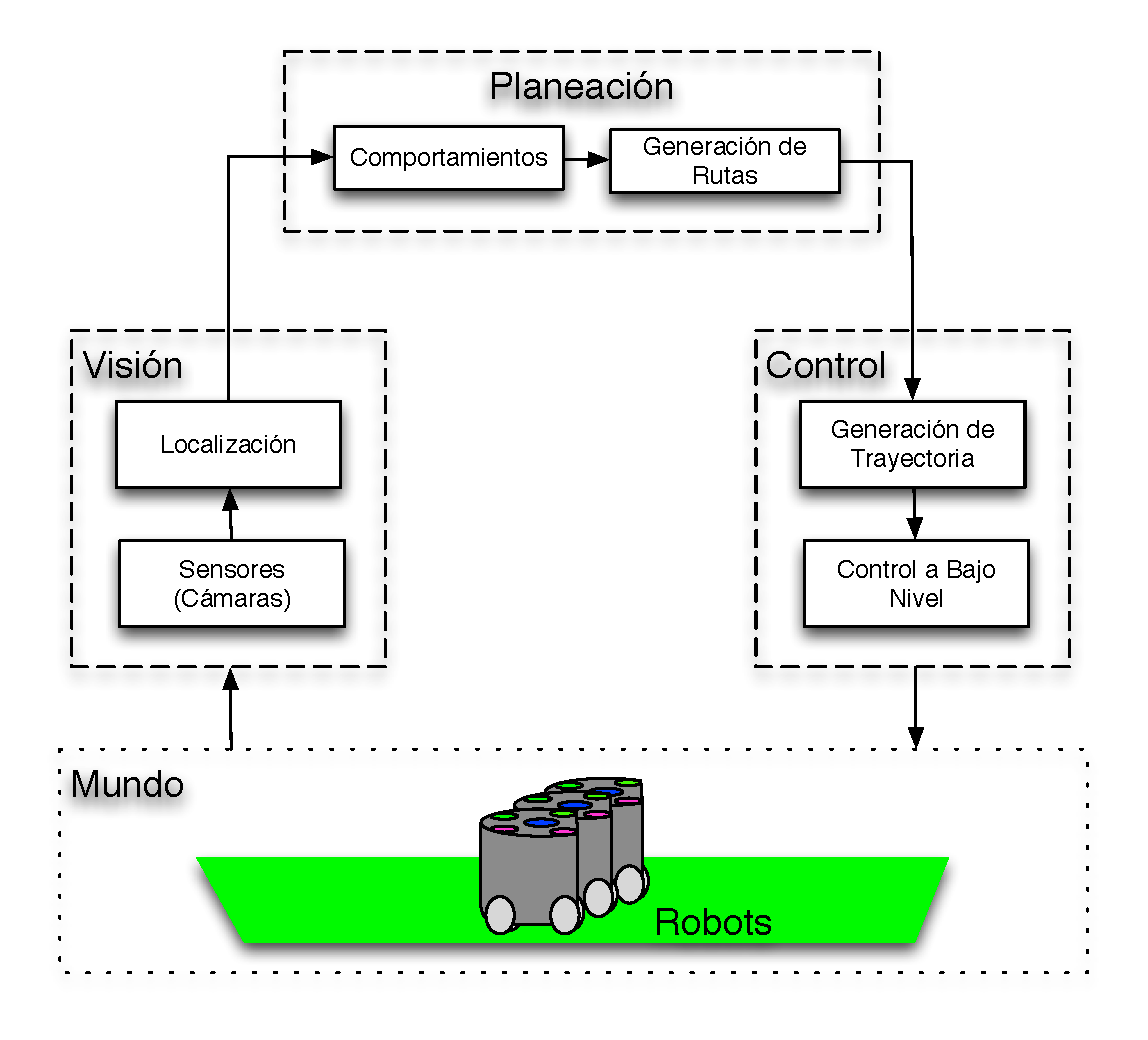
\includegraphics[scale=.5]{arqGeneral.eps}
  \caption{Arquitectura del Sistema}
  \label{fig:ROSGral}
\end{figure}
% \TODO{MM: si te da tiempo cambia las etiquetas ROS de los módulos de arriba y de la derecha por Planificación (la primera) y Control la Segunda}
%%%%%%%%%%%%%%%% end figure %%%%%%%%%%%%%%%%%%% 
\subsection*{Visión}
Este componente proporcionado por RoboCup SSL procesa las imágenes obtenidas de dos cámaras colocadas en la parte superior de la cancha para obtiener la pose de cada robot así como la posición de la pelota. Como el componente no está implementando en ROS, se implementó una interfaz para ROS que permite comunicarlo con los demás componentes.

%%%%%%%%%%%%%%%%%%%%%%%%%%%%%%%%%%%%%%%%%%%%%%%%%%%%%%%%%%%%%%%%%%%%%%
\subsection*{Planificación}
Este componente es el encargado de realizar la planificación de tareas y de movimientos para todos los robots de un equipo. La planificación de tareas se encarga de asignar poses meta a cada robot en base a un rol que tengan asignado. La planificación de movimientos identifica rutas libres de colisión para que cada robot llegue a la pose asignada por el planificador de tareas.
%%%%%%%%%%%%%%%%%%%%%%%%%%%%%%%%%%%%%%%%%%%%%%%%%%%%%%%%%%%%%%%%%%%%%%
\subsection*{Control}
El control está dividido en un generador de trayectorias y en un controlador de bajo nivel. Las trayectorias se generan para mover al robot de su pose actual a la deseada en el tiempo establecido por el planificador. De no ser posible generar la trayectoria deseada en el tiempo deseado, se reporta al planificador. La trayectoria resultante se discretiza y se envía al robot en forma de un perfil de velocidades en $x$, $y$ y $\theta$. 
 
%%%%%%%%%%%%%%%%%%%%%%%%%%%%%%%%%%%%%%%%%%%%%%%%%%%%%%%%%%%%%%%%%%%%%%
\subsection*{Partes físicas del robot}
Las partes físicas del robot incluyen su estructura interna, la electrónica de control y comunicaciones, los motores y las ruedas.

\subsubsection*{Estructura} La estructura del robot está limitada por las características definidas por la \textit{Small Size League} de la RoboCup. Debe caber dentro de un cilindro de 18 cm de altura por 15 cm de diámetro, siendo el diseño más eficiente un robot cilíndrico con ruedas concéntricas.
Realizando un análisis de los robots de la liga, se estableció la velocidad máxima en 3.5 m/s. Igualmente, la carga que debe soportar se estableció en 2.5 Kg. Por otro lado, debido a la velocidad del juego, es común que ocurran colisiones entre ellos por lo que el exterior del robot debe ser de un material resistente además contar con piezas fácilmente reemplazables. Por esto se optó por utilizar el modelado por deposición fundida (impresión 3D) con la ventaja de que este método permite realizar diseños complejos que se pueden probar rápidamente. Se utilizaron dos tipos de plástico: ABS y HIPS. El diseño modular resultante facilita adaptarlo a otros escenarios ásí como hacer mejoras. 

Los principales componentes de la estructura son la base y la carcasa. La base es la pieza en la cual se ensambla el resto de los componentes, mientras que la carcasa protege al robot de impactos. Estas piezas constituyen las piezas de mayores dimensiones en el diseño por lo que son manufactaras usando plástico HIPS al ofrecer mejores resultados en piezas de grandes dimensiones. La carcasa est\'a formada por 4 piezas \'unicas. En la parte superior de la carcasa se reservó un espacio donde se coloca el \textit{patrón estándar} necesario para que la visi\'on detecte la pose del robot.

\subsubsection*{Electrónica} Como se observa en la Figura \ref{fig:electGral}, la electrónica del robot se compone de una tarjeta de desarrollo MOJO, un sistema de comunicaciones y circuitos de fuente de energía y potencia para los motores. La tarjeta MOJO cual tiene una FPGA Spartan 6 XC6SLX9 descrita en la Sección~\ref{sec:fpga} y un microcontrolador ATmega32U4 que se describe en la Sección~\ref{sec:micro}. Para las comunicaciones se utiliza una tarjeta XBee WiFi como se describe en la Sección~\ref{sec:comunicaciones}. 
%%%%%%%%%%%%%%%% begin figure %%%%%%%%%%%%%%%%%%%
\begin{figure}
  \centering
    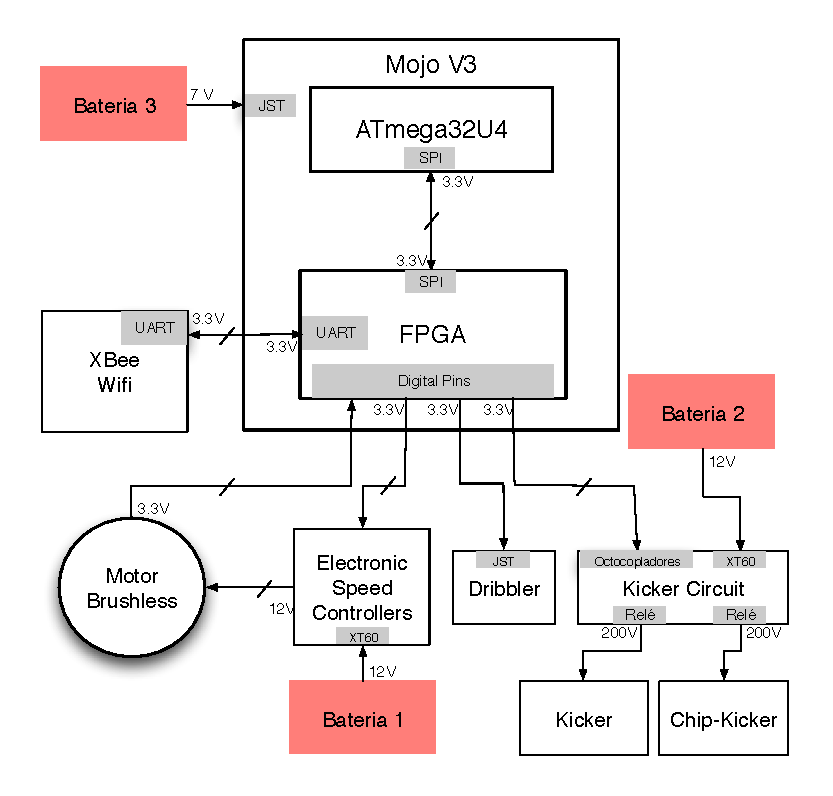
\includegraphics[width=8cm]{diagElectronica.eps}
  \caption{Componentes electrónicos}
  \label{fig:electGral}
\end{figure}
%%%%%%%%%%%%%%%% end figure %%%%%%%%%%%%%%%%%%%


Para dar potencia a cada motor se utiliza un ESC (Electronic Speed Controller) que sirve de interfaz entre la FPGA que envía una señal PWM y el motor. Este componente permite aislar eléctricamente la FPGA (que utiliza voltaje TTL) de los motores (12V) y transformar la señal de CD que proviene del PWM a una señal trifásica que requieren los motores sin escobillas utilizados. Se utiliza un modelo de ESC dedicado a drones multi-hélice debido a su rapidez de respuesta. 

Los mecanismos para el movimiento, motores y ESC son alimentados por una batería de 12 V. Los componentes que requieren de electricidad para funcionar son tres: mecanismos para el movimiento, para la pelota y el cómputo. Cada uno utiliza su propia batería LiPo para tenerlos aislados eléctricamente entre si, para la comunicación entre ellos se utilizan optocopladores. 


%%%%%%%%%%%%%%%%%%%%%%%%%%%%%%%%%%%%%%%%%%%%%%%%%%%%%%%%%%%%%%%%%%%%%%
\subsubsection*{Motores y reductores}
El motor utilizado es Maxon 200142. Este motor tiene una velocidad sin carga de 4370 RPM (nominal de 2940 RPM). Dados los requerimientos de velocidad y peso establecidos, es necesario utilizar un reductor de velocidad de 2.5. Se utilizó un reductor conformado por engranes cilíndricos rectos de metal. Se utilizan engranes comerciales debido a la necesidad de contar con alta eficiencia en la transmisión de la energía y ser resistentes en altas velocidades.


%%%%%%%%%%%%%%%%%%%%%%%%%%%%%%%%%%%%%%%%%%%%%%%%%%%%%%%%%%%%%%%%%%%%%%
\subsubsection*{Ruedas}
La mayoria de los diseños de ruedas omnidireccionales comerciales maximizan la eficiencia de la rueda buscando que el perfil de la rueda se perfectamente circular (\cite{rojas2005short}), sacrificando el espacio utilizado por la rueda. Debido a las restricciones en las dimensiones del robot, se realizó un diseño propio, delgado y con rodillos perpendiculares al eje principal.

Los factores más importantes en el diseño de la rueda es la facilidad de ser ensamblada y la resistencia del material utilizado. El diseño final utiliza cuatro piezas únicas, de las cuales 2 son de diseño propio: una pieza de plástico ABS (\ref{fig:ruedaOmni}) y 21 rodillos de aluminio; y dos piezas comerciales: 1 cable de acero y 21 orings. De esta manera, el esqueleto es formado por una pieza lo cual simplifica el ensamblado y la hace más resistente que otras versiones que utilizan varias piezas como esqueleto. Adicionalmente, el radio de la rueda así como el número de rodillos utilizados favorece un funcionamiento eficiente de la rueda comparado con versiones de menor tamaño o menor número de rodillos.

%%%%%%%%%%%%%%%% begin figure %%%%%%%%%%%%%%%%%%%
\begin{figure}[t]
  \centering
    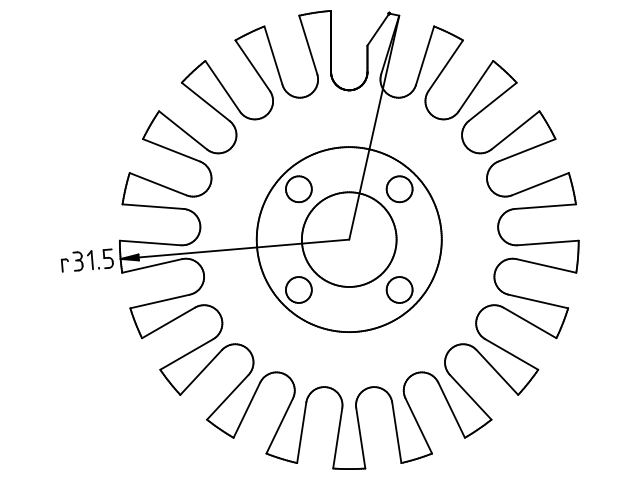
\includegraphics[scale=0.2]{rueda.png}
  \caption{Diagrama de la Rueda Omnidireccional Utilizada}
  \label{fig:ruedaOmni}
\end{figure}
%%%%%%%%%%%%%%%% end figure %%%%%%%%%%%%%%%%%%% 
%%%%%%%%%%%%%%%%%%%%%%%%%%%%%%%%%%%%%%%%%%%%%%%%%%%%%%%%%%%%%%%%%%%%%%
%%%%%%%%%%%%%%%%%%%%%%%%%%%%%%%%%%%%%%%%%%%%%%%%%%%%%%%%%%%%%%%%%%%%%%
%%%%%%%%%%%%%%%%%%%%%%%%%%%%%%%%%%%%%%%%%%%%%%%%%%%%%%%%%%%%%%%%%%%%%%
% \subsection*{Mecanismos para la Pelota}
% En esta sección se presentan los mecanismos diseñados para tener control de la pelota (\textit{dribbler}) así como el mecanismo de pateo (\textit{Kicker}).
% %%%%%%%%%%%%%%%%%%%%%%%%%%%%%%%%%%%%%%%%%%%%%%%%%%%%%%%%%%%%%%%%%%%%%%
% %%%%%%%%%%%%%%%% begin figure %%%%%%%%%%%%%%%%%%%
% \begin{figure}
%   \centering
%     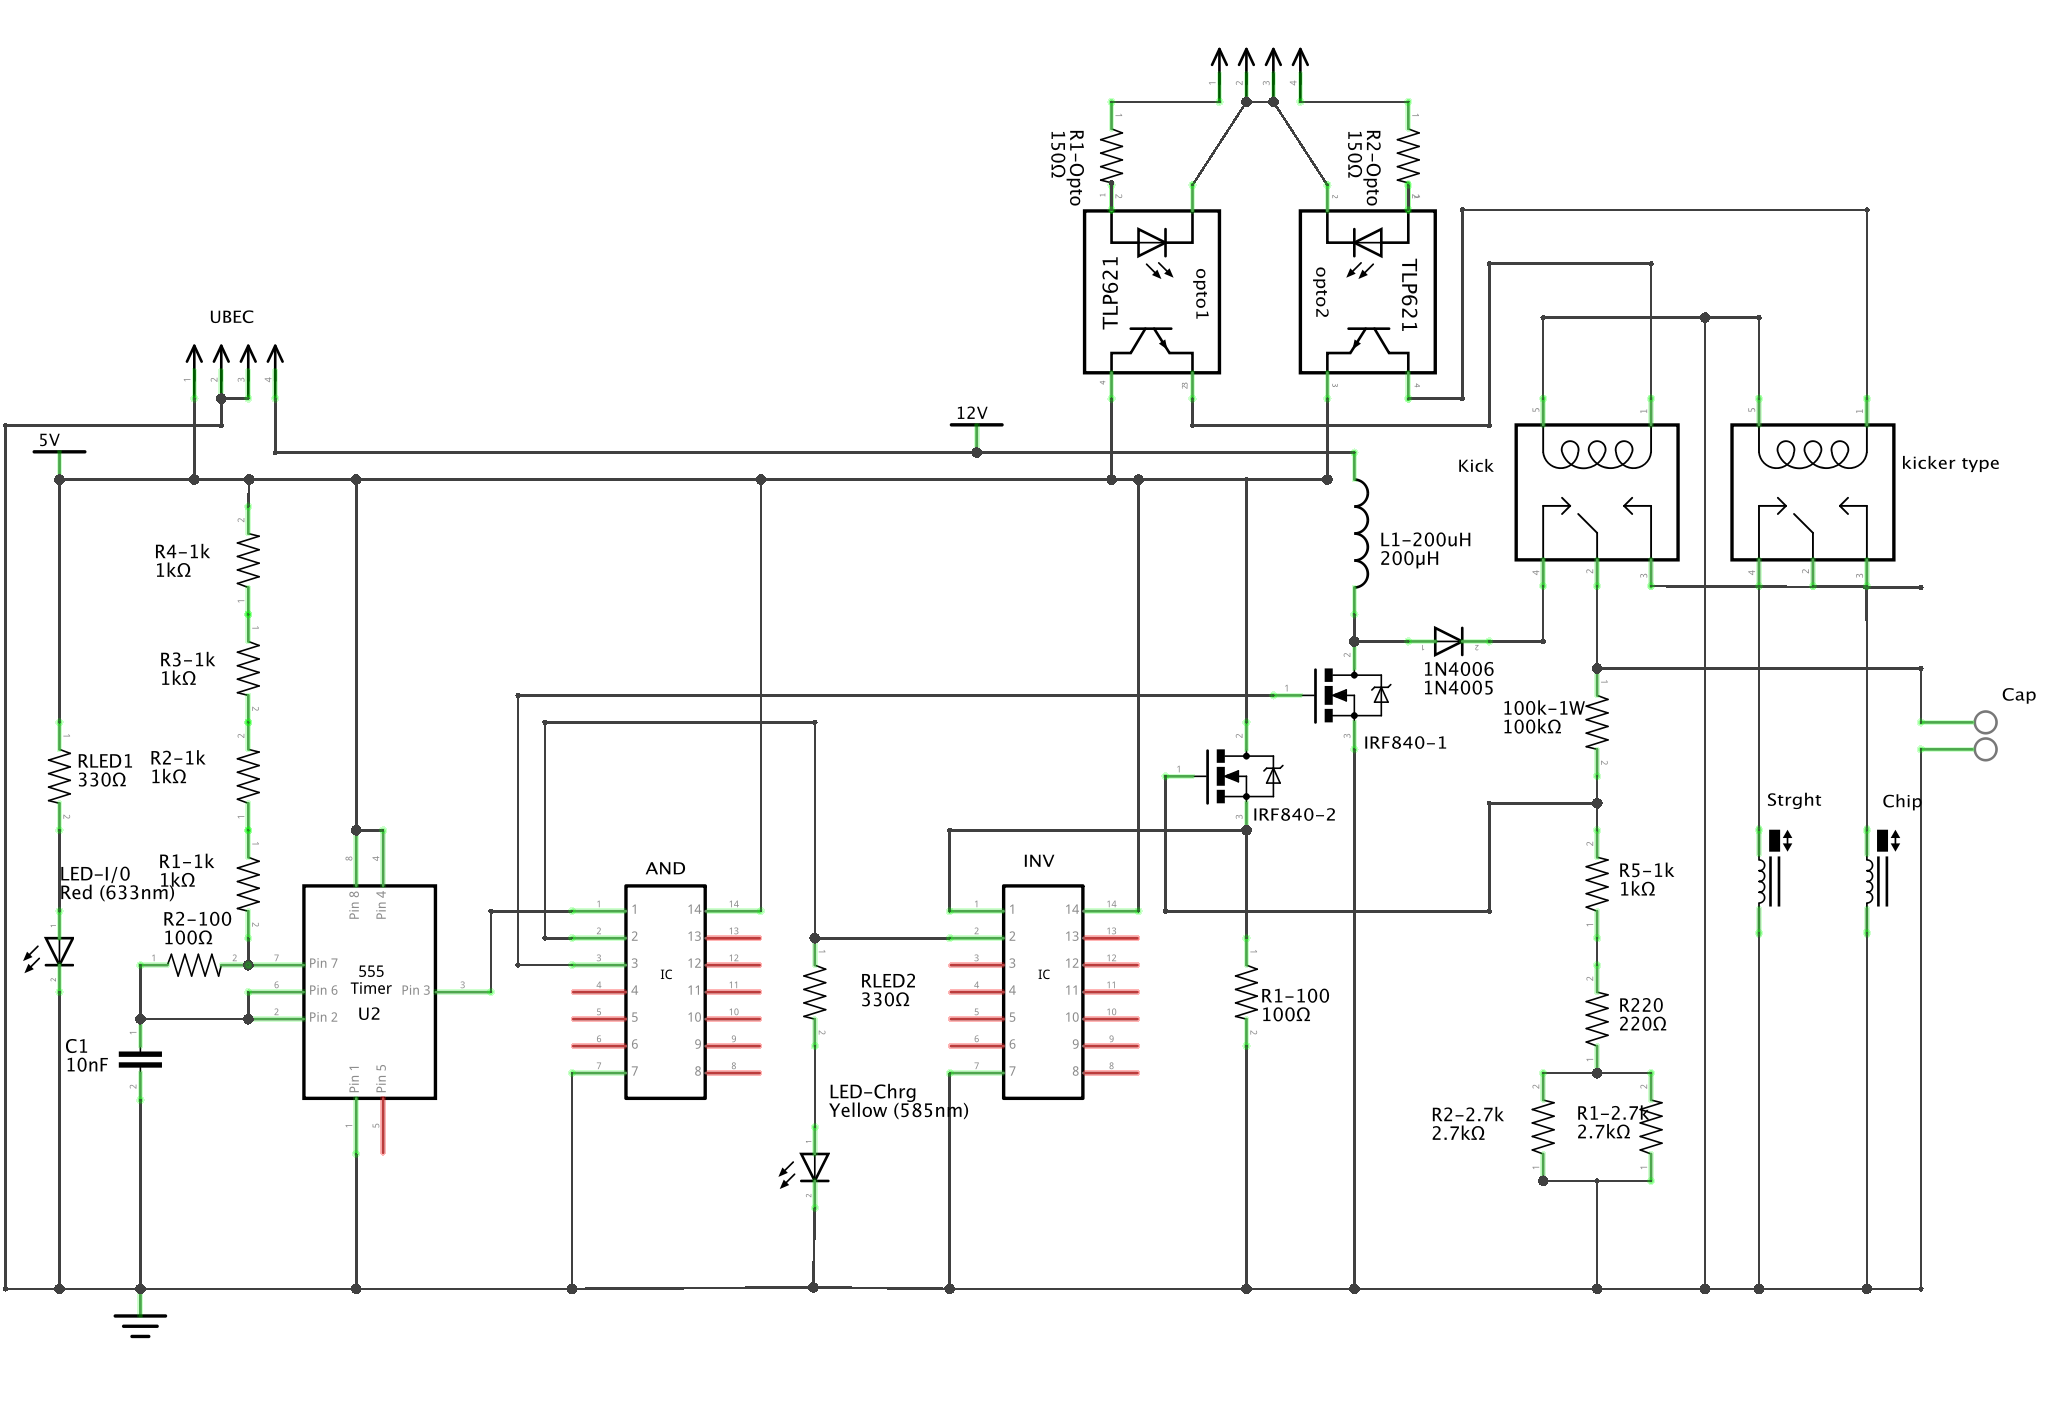
\includegraphics[width=8cm]{circuitoKicker.png}
%   \caption{Circuito para el Kicker}
%   \label{fig:elecKicker}
% \end{figure}
% %%%%%%%%%%%%%%%% end figure %%%%%%%%%%%%%%%%%%%
% %%%%%%%%%%%%%%%%%%%%%%%%%%%%%%%%%%%%%%%%%%%%%%%%%%%%%%%%%%%%%%%%%%%%%%
% \subsubsection*{Kickers}
% Se utiliza un seleonoide el cual es alimentado con 200 V cuando se da la señal para patear. En la Fig. \ref{fig:elecKicker} se muestra el circuito utilizado para llevar la entrada de 12 V a una salida de 200 V. Dentro del circuito, se utiliza un \textit{Universal Battery Elimination Circuit (UBEC)} para alimentar con 5 V los circuitos integrados a partir de los 12 V de la batería. \par
% %%%%%%%%%%%%%%%%%%%%%%%%%%%%%%%%%%%%%%%%%%%%%%%%%%%%%%%%%%%%%%%%%%%%%%
% \subsubsection*{Dribbler}
% El mecanismo del dribbler consiste en un motor DC que funciona entre 3 y 5 V así como un sistema de engranes de plástico para la transimisión de energía y una espuma en el punto de contacto con la pelota. Para el control del dribbler se utiliza un Puente H en modo unidireccional. \par 
% Para el dribbler, se utiliza un Puente H en modo unidireccional para controlar un motor DC. \par
%%%%%%%%%%%%%%%%%%%%%%%%%%%%%%%%%%%%%%%%%%%%%%%%%%%%%%%%%%%%%%%%%%%%%%
% \subsubsection*{DRIVER}

%%%%%%%%%%%%%%%%%%%%%%%%%%%%%%%%%%%%%%%%%%%%%%%%%%%%%%%%%%%%%%%%%%%%%%
\subsubsection*{FPGA}
\label{sec:fpga}
Debido a que es necesario controlar los 4 motores así como otros componentes, es necesario atender simultaneamente múltiples entradas y salidas. Una FPGA ofrece esta capacidad además de permitir representar números con mayor resolución que un microcontrolador. En el sistema implementado, la FPGA tiene seis funciones:
\begin{enumerate}
  \item Recibir los datos del XBee.
  \item Calcular la velocidad de cada motor mediante la señal de cada sensor hall.
  \item Mandar la velocidad deseada a cada ESC mediante PWM.
  \item Activar el dribbler.
  \item Activar el kicker.
  \item Recibir y procesar señales de sensores adicionales.
\end{enumerate}
La FPGA se comunica con el Microcontrolador mediante SPI y Memory Mapping. Envía las velocidades deseadas $(V_x,V_y,\omega)$ así como las velocidades reales de cada motor y recibe las velocidades deseadas para cada motor.\par

%%%%%%%%%%%%%%%%%%%%%%%%%%%%%%%%%%%%%%%%%%%%%%%%%%%%%%%%%%%%%%%%%%%%%%
\subsubsection*{Microcontrolador}
\label{sec:micro}
En cada ciclo del microcontrolador, se reciben las velocidades deseadas $(V_x,V_y,\omega)$ así como las reales de cada motor y se determina una nueva velocidad deseada mediante el modelo omnidireccional. Las velocidades por motor calculadas son transferidas a la FPGA. El modelo cinemático del robot así como el algoritmo de control son implementados en el microcontrolador como se describe en la Sección~\ref{sec:algoritmos}.
% En cada ciclo, se leen los registros de las velocidades de cada motor (deseada y real) y se realizan los cálculos para determinar la nueva velocidad de cada motor de acuerdo a los modelo omnidireccional y al algoritmo de control utilizado. \par

%%%%%%%%%%%%%%%%%%%%%%%%%%%%%%%%%%%%%%%%%%%%%%%%%%%%%%%%%%%%%%%%%%%%%%
\subsubsection*{Comunicación}
\label{sec:comunicaciones}
Para el control del robot es necesario contar con comunicación inalámbrica. Se eligió WiFi porque se puede utilizar prácticamente cualquier equipo de cómputo para el control del robot. En específico, se utiliza XBee WiFi por su tamaño con voltajes TTL compatibles con la FPGA. Se utiliza direccionamiento estático para tener control de las IPs de cada robot, además de facilitar la conexión inicial con el access point. Para favorecer un diseño modular, el resto de los componentes son agnósticos a la tecnología utilizada para la comunicación. \par %El robot es capaz de reportar las velocidades deseadas calculadas mediante WiFi con fines de \par
% Aunque existen diversos métodos de comunicación inalámbrica, se decidió utilizar WiFi debido a la facilidad de adaptar cualquier computadora para ser utilizada con el robot. En el robot se utiliza un radio XBee Wifi debido a las diversas facilidades que ofrece la plataforma de XBee además de ser conveniente su tamaño y alimentación (3.3V). \par


%%%%%%%%%%%%%%%%%%%%%%%%%%%%%%%%%%%%%%%%%%%%%%%%%%%%%%%%%%%%%
\section*{ALGORITMOS}
\label{sec:algoritmos}
En esta sección se describen los algoritmos implementados en el robot para su control de bajo nivel.

\subsection*{Movimiento Omnidireccional}
%%%%%%%%%%%%%%%% begin figure %%%%%%%%%%%%%%%%%%%
\begin{figure}
  \centering
    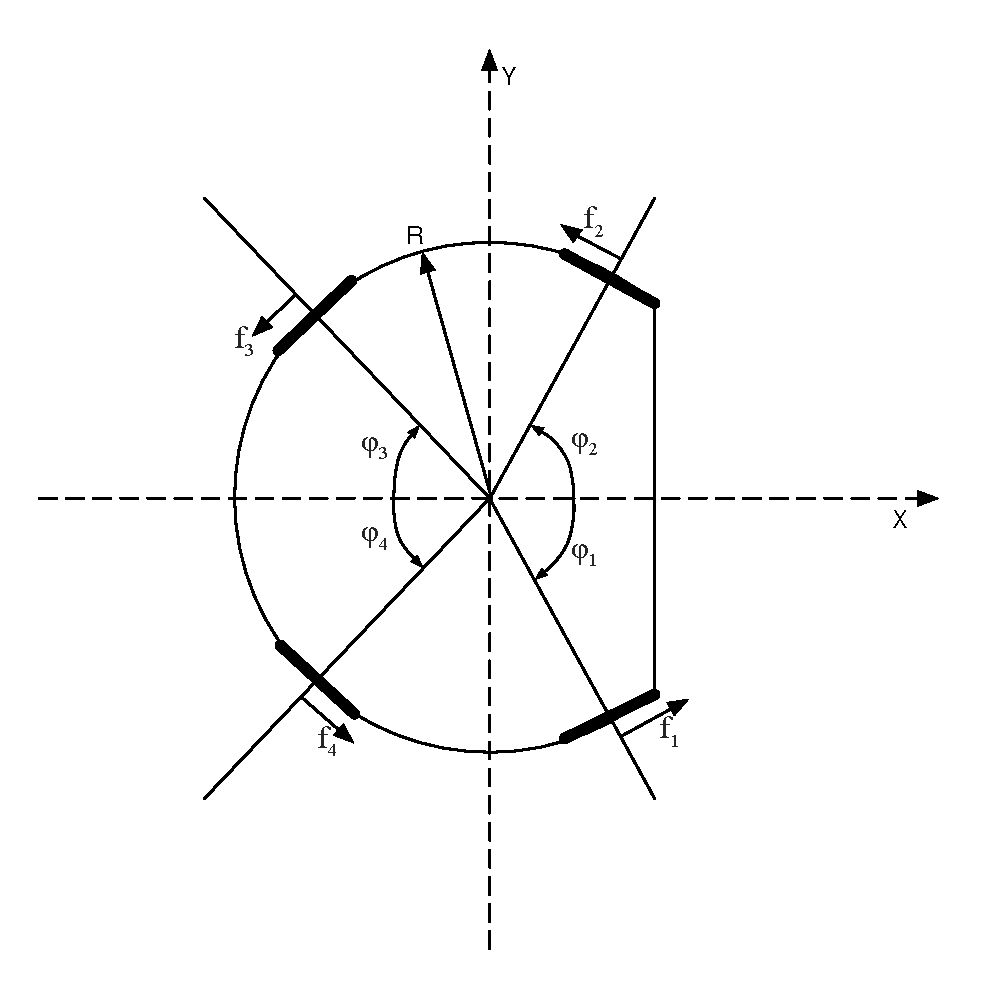
\includegraphics[scale=0.4]{anglesRobot.eps}
  \caption{Distribución de Ángulos y Fuerzas}
  \label{fig:angFzaDiag}
\end{figure}
%%%%%%%%%%%%%%%% end figure %%%%%%%%%%%%%%%%%%%
El movimiento deseado para el robot se expresa en un vector de velocidades deseadas \( V_l= \begin{pmatrix} v_x & v_y & \omega \end{pmatrix}^{T} \) que es necesario descomponer en velocidades de motores deseadas \( V_m= \begin {pmatrix} m_1 & m_2 & m_3 & m_4 \end{pmatrix}^{T} \). 

A partir de la ecuación general de fuerza \( F = Ma \) se deriva la Ecuación~(\ref{eq:fmaMots}) específica para el caso de cuatro motores. Debido a las ruedas omnidireccionales, cada motor aporta en los componentes de $X$ y $Y$. En base al diagrama de la Fig. \ref{fig:angFzaDiag}, se observa que para el motor 1 la aportación es descrita por las ecuaciones ~(\ref{eq:max1}) para $X$ y ~(\ref{eq:may1}) para $Y$. Similarmente, se pueden obtener las ecuaciones para los otros motores.
%%%%%%%%%%%%%%%% Equation %%%%%%%%%%%%%%%%%%
% \begin{equation}
%   F= Ma \label{eq:FMA} \\
% \end{equation}
\begin{equation}
  a = \frac{1}{M}\left(F_1+F_2+F_3+F_4\right) \label{eq:fmaMots} \\
\end{equation}
%%%%%%%%%%%%%% End Equation %%%%%%%%%%%%%%%%
\begin{equation}
  Ma_{1x} = \mid f_1 \mid \cos\left(90 - \varphi_1\right) =  \mid f_1 \mid  \sin\left(\varphi_1\right)\label{eq:max1}
\end{equation}
\begin{equation}
  Ma_{1y} = \mid f_1 \mid \cos\left(\varphi_1\right) \label{eq:may1}
\end{equation}
% \begin{equation}
%   Ma_{2x} = - \mid f_2 \mid  \sin\left(\varphi_2\right)
% \end{equation}
% \begin{equation}
%     Ma_{2y} = \mid f_2 \mid \cos\left(\varphi_2\right) 
% \end{equation}
% \begin{equation}
%   Ma_{3x} = - \mid f_3 \mid  \sin\left(\varphi_3\right)
% \end{equation}
% \begin{equation}
%     Ma_{3y} = \mid f_3 \mid \cos\left(\varphi_3\right)
% \end{equation}
% \begin{equation}
%   Ma_{4x} = \mid f_4 \mid  \sin\left(\varphi_4\right) 
% \end{equation}
% \begin{equation}
%     Ma_{4y} = \mid f_4 \mid \cos\left(\varphi_4\right)  \label{eq:Ma-xy234}\\
% \end{equation}

Para obtener la aceleración angular que aporta cada motor al robot, de la Eqn. \(\dot{\omega} = \frac{Rf}{I}\) se puede derivar la Eqn.~(\ref{eq:omega4Mots}) específica para el uso de 4 motores. Sustituyendo el momento de inercia Eqn.~(\ref{eq:inercia}) para el caso de un cilindro con distribución de masa desconocida en (\ref{eq:omega4Mots}) se obtiene la Eqn.~(\ref{eq:Romega}). \par

% \begin{equation}
%   \dot{\omega} = \frac{Rf}{I} \label{eq:omegaGral} 
% \end{equation}
\begin{equation}
  \dot{w} =\frac{R}{I}\left(f_1+f_2+f_3+f_4\right) \label{eq:omega4Mots}
\end{equation}
\begin{equation}
  I = \alpha M R^{2} ;\qquad 0\leq \alpha \leq1 \label{eq:inercia}
\end{equation}
\begin{equation}
  R\dot{\omega} = \frac{1}{M\alpha}\left(f_1+f_2+f_3+f_4\right) \label{eq:Romega}
\end{equation}

De los resultados obtenidos de las aceleraciones traslacionales y angulares, se puede derivar la Eqn.~(\ref{eq:matAcoFzas}). Tambien se puede expresar como \(a=C_\alpha F \), donde \( C_\alpha \) se conoce como la Matriz de Acoplamiento de Fuerzas. \par

% Matriz de Acoplamiento de Fuerzas
\begin{equation}
  \left(\begin{array}{c}
    a_x \\ a_y \\R_{\dot{\omega}}
  \end{array}\right)= \frac{1}{M}
  \begin{bmatrix}
    \sin\varphi_1 & -\sin\varphi_2 & -\sin\varphi_3 & \sin\varphi_4 \\
    \cos\varphi_1 & \cos\varphi_2 & -\cos\varphi_3 & -\cos\varphi_4 & \\
    \frac{1}{\alpha} & \frac{1}{\alpha}  & \frac{1}{\alpha}  &\frac{1}{\alpha} 
  \end{bmatrix}
  \left(\begin{array}{c}
    f_1 \\ f_2 \\ f_3 \\ f_4  \label{eq:matAcoFzas}\\ 
  \end{array}\right) 
\end{equation}
% \begin{equation}
%   a=C_\alpha F \label{eq:gralAcoFzas} \\
% \end{equation}

Para transformar la velocidad deseada en el espacio a velocidades de cada motor, es necesario considerar el perímetro de la rueda y el factor de reducción mediante \(V_{l}^{'} = \frac{ V_l \cdot e } { 2 \pi r} \). Así, se obtienen las ecuaciones de cada motor mediante la Eqn. \eqref{eq:velsMots}  y su forma reducida \(v_m = D V_{l}^{'}\) donde a \( D \) se le conoce como la Matriz de Acoplamiento de Velocidades. \par 

% \begin{equation}
%   V_{l}^{'} = \frac{ V_l \cdot e } { 2 \pi r} \label{eq:reductorPerim}
% \end{equation}
\begin{equation}
  % v_1 = v_x \sin\varphi_1 + v_y\cos\varphi_1 + R \omega \label{eq:velMot1}\\
  v_m = 
    \left(\begin{array}{c}
      v_1 \\ v_2 \\ v_3 \\ v_4 
    \end{array}\right)
    = 
    \begin{bmatrix}
      \sin\varphi_1 & \cos\varphi_1 & 1 \\
      -\sin\varphi_2 & \cos\varphi_2 & 1 \\
      -\sin\varphi_3 & -\cos\varphi_3 & 1 \\
      \sin\varphi_4 & -\cos\varphi_4 & 1 \\
    \end{bmatrix}
    \left(\begin{array}{c}
      v_x^{'}  \\ v_y^{'}  \\ {Rw}^{'} 
    \end{array} \right) \label{eq:velsMots} \\
\end{equation}
% \begin{equation}
%     v_m = D V_{l}^{'} \label{eq:velsMotsReduce} \\
% \end{equation}
\par

% Gracias a la retroalimentación obtenida de cada motor, es posible calcular la velocidad real \( V_{l}^{r} \) a la cual se está moviendo cada motor. Además, es posible determinar la velocidad real del robot. A partir de la ecuación \eqref{eq:velsMotsReduce}, definiendo \( D^{+} \) como la una pseudoinversa de D tal que la identidad \eqref{eq:DsToIdent} se cumple y definiendo el vector \( v_m^{r} = \begin{pmatrix}v_1^{r} & v_2^{r} & v_3^{r} & v_4^{r} \end{pmatrix}^{T} \), se obtiene la identidad \eqref{eq:velsMotToVelsRob}. \par

% \begin{equation}
%   D^{+}D = I_3 \label{eq:DsToIdent}
% \end{equation}
% \begin{equation}
%   V_{l}^{r} = D^{+}v_m \label{eq:velsMotToVelsRob} b
% \end{equation}

% Para el caso específico en el que \(  \varphi_1 = \varphi_2 \) y \(  \varphi_3 = \varphi_4 \), la pseudoinversa es la siguiente:

% \begin{equation}
%   D^{+} = \begin{bmatrix}a & -a &-c & c \\e & e & -g & -g \\ i & i & k & k \end{bmatrix} \\
% \end{equation}
% Donde:
% \begin{equation}
%   \begin{aligned}
%   a & = c \cdot \cos \varphi_1  & \qquad k & = \frac{1}{\frac{2\cos \varphi_3}{\cos \varphi_1} + 2} \\
%   c & = \frac{1}{\frac{2 (\cos \varphi_3)(\sin \varphi_1) }{\cos \varphi_1} + 2\sin\varphi_3} & e & = \frac{1}{2(\cos \varphi_1 + \cos \varphi_3)} \\ 
%   i & = \frac{k \cdot \cos \varphi_3}{\cos \varphi_1} & g & = e \\
%   \end{aligned}
% \end{equation}
%%%%%%%%%%%%%%%%%%%%%%%%%%%%%%%%%%%%%%%%%%%%%%%%%%%%%%%%%%%%%%%%%%%%%%
%%%%%%%%%%%%%%%% begin figure %%%%%%%%%%%%%%%%%%%
\begin{figure}
  \centering
    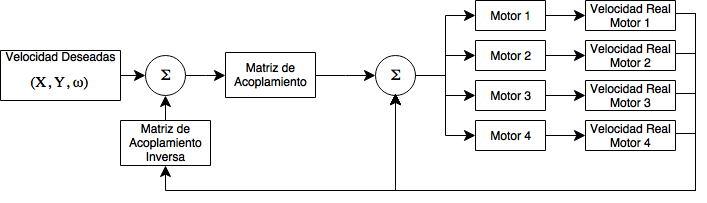
\includegraphics[width=8cm]{ciclo_ctrl_avr.png}
  \caption{Esquema de Control Implementado}
  \label{fig:ctrl}
\end{figure}
%%%%%%%%%%%%%%%% end figure %%%%%%%%%%%%%%%%%%% 
%%%%%%%%%%%%%%%%%%%%%%%%%%%%%%%%%%%%%%%%%%%%%%%%%%%%%%%%%%%%%%%%%%%%%%
\subsection*{Control}
Para el control, se implementó un control PI a nivel de cada motor. El esquema general del algoritmo de control utilizado se muestra en la Fig. \ref{fig:ctrl}. La sintonización de las variables se realiza a mano siguiendo el método de Ziegler - Nicholson. \par
% Se incorporó un PI a nivel motor, utilizando el método de Ziegler - Nicholson para realizar la sintonización de las variables.
Adicionalmente, se cuenta con la retroalimentación de la visión gracias a la cual se puede calcular y corregir la trayectoria del robot al enviar continuamente actualizaciones de la velocidad deseada (30 Hz). 
% En la Fig. \ref{fig:visionPrueba} se muestran las trayectorias seguidas por el robot al utilizar solamente el control PI así como utilizando el control PI y la retroalimentción de la visión.

%%%%%%%%%%%%%%%%%%%%%%%%%%%%%%%%%%%%%%%%%%%%%%%%%%%%%%%%%%%%%%%%%%%%%%
%%%%%%%%%%%%%%%% begin figure %%%%%%%%%%%%%%%%%%%
\begin{figure}
  \centering
    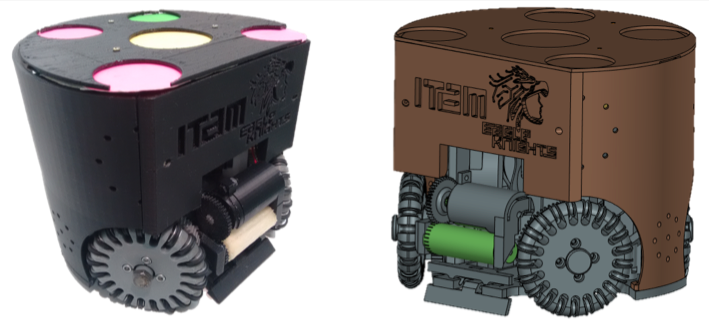
\includegraphics[height=3cm,width=8cm]{realVS3D.png}
  \caption{Robot Real vs Modelo 3D del Robot}
  \label{fig:ModRealVSdes}
\end{figure}
%%%%%%%%%%%%%%%% end figure %%%%%%%%%%%%%%%%%%% 

%%%%%%%%%%%%%%%%%%%%%%%%%%%%%%%%%%%%%%%%%%%%%%%%%%%%%%%%%%%%%%%%%%%%%%
\section*{EXPERIMENTACIÓN Y RESULTADOS}
% Con el diseño propuesto se logra que el robot se mueva aproximadamente a la velocidad propuesta, manteniendo la integridad de sus componentes y con un peso menor que el contemplado inicialmente, aunque siendo capaz de cargar los 3.5 Kg propuestos. Tanto la carcasa como la base y las ruedas han sido capaces de resistir golpes entre los robots a las velocidades normales de movimiento y la visión reconoce el patrón estandar incoporado en la carcasa. En la Fig. \ref{fig:ModRealVSdes} se muestra una comparación entre el diseño modelado en 3D y la construcción final del robot.\par 
\EXCISE{
  En la Fig. \ref{fig:realVSdes} se puede ver la respuesta de un motor ante una velocidad deseada con el algoritmo de control PI implementado. Aunque las oscilaciones no se eliminan, se reducen rápidamente, siendo la respuesta rápida uno de los factores más importantes debido al dinamismo del sistema. Igualmente, el motor es capaz de cambiar de velocidad, incluso a velocidades negativas (dirección contraria) rápidamente.

  Estableciendo 8 direcciones en el plano XY, se obtuvo la respuesta del robot en cada dirección con control PI sin visión y con visión como se puede ver en la Fig. \ref{fig:visionPruebasRetro}. Para el caso del robot sin retroalimentación de visión, existen algunas direcciones en las cuales el movimiento y su posición final es cercano al deseado, especificamente en las direcciones en que prácticamente sólo se utilizan dos ruedas. En cambio en las otras direcciones, se tiene mayor error en el movimiento del robot. Para el caso del movimiento con retroalimentación de visión, aunque en algunos casos existe un movimiento errático, la posición final es muy cercana a la deseada gracias a la correción que realiza el sistema ante los errores en el movimiento del robot.

  Utilizando los datos del experimento anterior, se obtener el error en el tiempo definido como la diferencia entre la posición deseada y la medida, en la Fig. \ref{fig:errorPlot} se puede observar la mejora que representa la retroalimentación de visión. Se puede observar como el error en las trayectorias sin visión es incremental mientras que en las trayectorias con visión, el error alcanza un máximo para disminuir, alcanzando la posición deseada.
}
Para validar el desempeño de los motores ante una entrada de velocidad deseada del robot, se definen 3 velocidades posibles para cada componente del vector $(X, Y, \theta ): +V_{cte}, 0, -V_{cte}. $  Existen 27 posibles combinaciones. En la Fig. \ref{fig:realVSdes} se muestra la respuesta de cada motor así como del vector de velocidad deseada del robot bajo dos esenarios distintos. Para el primer escenarios solamente se utiliza el lazo de control a nivel de motor. Para el segundo escenario se utiliza tanto el lazo de control a nivel de motor como el lazo de control a niver de robot. Durante la prueba, cada combinación es enviada al robot con un periodo de 10 segundos trasa el cual se apagan los motores por 10 segundos.
\par
En las pruebas para el primer escenario, la velocidad deseada de cada motor permanece constante una vez recibida la señal. Aunque en la mayoría de las combinaciones se alcanzan las velocidades de motor deseadas, resaltan 2 casos específicos. En el primero, en ciertas combinaciones como $(+V, +V, +V )$ y $(-V, -V, -V) $ para el motor 1, no se alcanza la velocidad deseada por ser mayor a la velocidad sin carga de 72 RPS. El segundo caso se presenta en combinaciones como $(+V, -V, 0) $ y  $(+V, -V, -V)$ , en las cuales la velocidad deseada para algún motor es muy baja para que el motor la pueda mantener por lo que comienza a oscilar alrededor de ésta. En ambos casos, el que uno o más motores no alcancen ni se mantengan en la velocidad deseada repercute en el vector de velocidades reales del robot: en ambos casos, no se alcanzan las velocidades deseadas pero en el segundo además se presenta una oscilación importante.
\par
En el segundo escenario, la velocidad deseada de motor no es constante ante cada entrada ya que es determinada por el ciclo de control a nivel robot. Aunque no siempre se alcanzan las velocidades deseadas por motor, sí se alcanzan y se mantienen las velocidades del vector $(X, Y, \theta )$. En algunos casos como $(+V, +V, +V )$ y $(+V, +V, -V) $, se tarda mucho en alcanzar la velocidad deseada aunque esto se puede mejorar utilizando otros valores $k_p$ y $k_i$.
\par

\NOTE{En la imagén \ref{fig:realVSdes} se podría cambiar a que sea solamente una entrada y su respuesta?}
%%%%%%%%%%%%%%%%%%%%%%%%%%%%%%%%%%%%%%%%%%%%%%%%%%%%%%%%%%%%%%%%%%%%%%
%%%%%%%%%%%%%%%% begin figure %%%%%%%%%%%%%%%%%%%
\begin{figure}
  \centering
    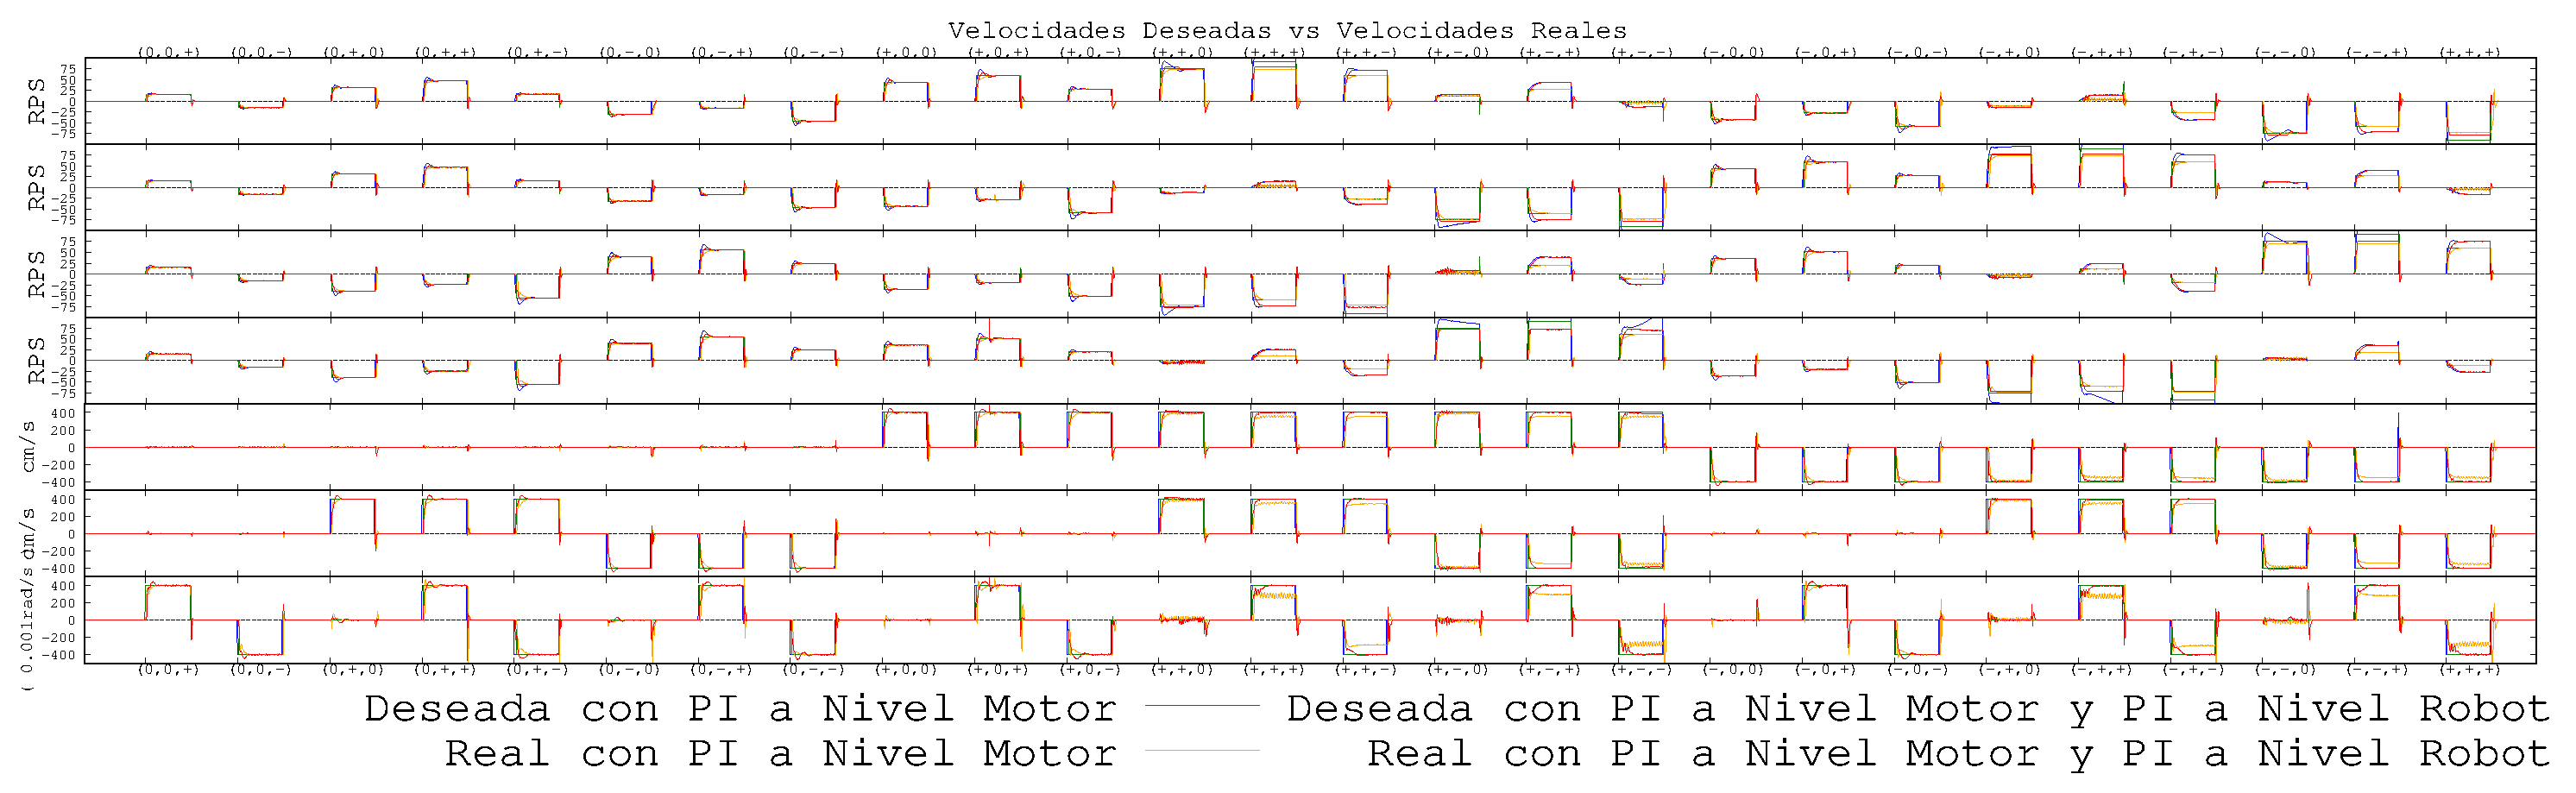
\includegraphics[height=3cm,width=8cm]{160517-vels-motVSmotrob.eps}
  \caption{Velocidad de Motor Real vs Velocidad de Motor Deseada}
  \label{fig:realVSdes}
\end{figure}
%%%%%%%%%%%%%%%% end figure %%%%%%%%%%%%%%%%%%% 
%%%%%%%%%%%%%%%%%%%%%%%%%%%%%%%%%%%%%%%%%%%%%%%%%%%
\subsection*{Prubas sin Retroalimentación de Visión}
\label{subsec:pruebas_sin_vision}
%%%%%%%%%%%%%%%%%%%%%%%%%%%%%%%%%%%%%%%%%%%%%%%%%%%%%

El objetivo de éstas pruebas es validar el movimiento omnidireccional del robot sin tener retroalimentaicón de ningún sistema externo. El sistema de Visión de SSL es utilizado para la captura de datos y generar la velocidad inicial deseada.
\par
Para las pruebas, se define una circunferencia con centro en un \textit{p0}. Se toman 8 puntos ${P_1, P_2, ..., P_8}$ en la circunferencia tales que: $\angle P_nP_0P_{n+1} = 45^\circ $. La prueba realizada consiste en colocar al robot en $P_0$, siempre orientado a $P_3$ y mandar solamente un mensaje con la velocidad deseada en dirección a uno de los 8 puntos. Solamente se da velociad en X y/o Y, manteniendo la velocidad de $\theta$ en 0. Con esto se busca probar que el robot es capaz de mantener su orientación al moverse en cualquier dirección. 
\par
La Fig. \ref{fig:8pts_without_vision} muestra la posición de los puntos $P_0, P_1, ..., P_8$ así como los vectores que idealmente seguiría el robot a cada punto. También se muestran las trayectorias reales seguidas por el robot en cada una de 10 repeticiones a cada punto. A partir de estos datos, se obtuvo una tendencia del movimiento del robot a cada punto. 
\par
Cada data de la trayectoria del robot representa la posición del centro del robot a un tiempo determinado. Por claridad, cada punto está representado con dimensiones menores a las del robot, el área que ocupa en realidad el robot es un círculo de 90 mm de radio; en la gráfica se muestra el un punto escala 1:1 en la esquina inferior derecha. Debido a las características particulares del sistema de visión, éste no reporta la posición del robot si se encuentra cercano al extremo derecho (donde se encuentra $P_3$) aunque el robot se encuentra en esa zona.
\par
%%%%%%%%%%%%%%%%%%%%%%%%%%%%%%%%%%%%%%%%
\subsubsection*{Movimiento en el Plano}
%%%%%%%%%%%%%%%%%%%%%%%%%%%%%%%%%%%%%%%%
La dirección que mejor desempeño mostró en estas pruebas fue $(+V, 0, 0)$ al punto 3. Aunque se tiene cierta varianza, en la mayoria de los casos el robot llega directo al punto 3 en linea prácticamente recta. La tendencia casi coincide don el vector que idealmente seguiría el robot. Para la dirección $(-V, 0, 0)$ a $P_7$ se presenta un desempeñomuy similar teniendo una clara desviación hacia el la dirección $+Y$ del eje coordenado del robot. El robot mantiene una trayectoria casi recta en la mayoria de los casos, la línea de tendecia pasa muy cerca de $P_7$.
\par
Las direcciones $(+V, -V, 0)$ y $(+V, +V, 0)$ a los puntos $P_2$ y $P_4$ respectivamente, presentan resultados muy similares. En ambos casos, las trayectorias del robot son curvas, cruzando al vector de dirección ideal. A pesar de ésto, la tendencia queda muy cercana al punto objetivo dentro de las dimensiones del robot. \par
Las direcciones $(-V, -V, 0)$ y $(-V, +V, 0)$ a los puntos $P_6$ y $P_8$ respetivamente, presentan errores importantes en las trayectorias. En estos dos casos, se observa la acción del ciclo de control a nivel robot al correjir el movimiento y llegar al punto objetivo. Las tendencias quedan muy cerca de los puntos objetivos aunque ambas atraviezan los vectores de dirección ideal. Especialmente la tendencia de las trayectorias al punto $P_6$ queda muy cercana al punto aunque existe una varianza importante. 
\par
Por último, las direcciones $(0, +V, 0)$ y $(0, -V, 0)$ a los puntos $P_1$ y $P_5$ son las que presentan el peor desempeño teniendo un error importante respecto al punto objetivo, no alcanzándolo en ninguna ocación. Las líneas de tendencia muestran una clara desviación respecto a los vectores de trayectoria ideal. Estos resultados reflejan la eficiencia de los valores utilizados para $k_p$ y $k_i$ del control PI, modificando estos valores se podrían obtener mejores resultados. 
\par
En la Fig. \ref{fig:8pts_without_vision} se puede observar que las trayectorias del robot parecen reflejarse alrededor del eje X. Al moverse solamente en ésta dirección es que el robot presenta mejores resultados. 
\par
%%%%%%%%%%%%%%%% begin figure %%%%%%%%%%%%%%%%%%%
\begin{figure}
  \centering
    \includegraphics[height=3cm,width=8cm]{8pts260517-without-vision.eps}
  \caption{Trayectorias con retroalimentación}
  \label{fig:8pts_without_vision}
\end{figure}
%%%%%%%%%%%%%%%% end figure %%%%%%%%%%%%%%%%%%%
%%%%%%%%%%%%%%%%%%%%%%%%%%%%%% 
\subsubsection*{Orientación}
%%%%%%%%%%%%%%%%%%%%%%%%%%%%%%
A partir de los mismos datos utilizados en la subsección pasada, en la Fig. \ref{fig:orient_without_vision}
se muestra el error en la orientación para cada prueba realizada a cada punto. Los datos presentan saltos debido a que solo se presenta la orientación durante el movimiento del robot de $P_0$ al punto deseado, no del reposicionamiento a $P_0$.
\par
La orientación del robot durante las trayectorias a los puntos $P_3$ y $P_7$ son las que menor error presentaron. Para los puntos $P_2, P_4, P_6$ y $P_8$, el error en la orientación es mayor aunque (salvo en dos pruebas) el error es menor a 0.5 radianes. Para estos casos, el error comienza en una dirección y generalmente existe una sobrecompensación de éste error llevandolo a la dirección contraria. La orientación en las trayectorias a los puntos $P_1$ y $P_5$, el error sobrepasa los 0.5 radianes en la mayoría de las pruebas, aunque es mayor en las trayectorias al punto $P_1$. 
\par
En error en la orientación del robot en las trayectorias a cada punto es consistente con el error en su movimiento en el plano. Los errores en la orientación también se reflejan en el eje X del robot: las direcciones del error para los puntos $P_1, P_2 $ y $P_8$ es la contraria que para los puntos $P_4, P_5$ y $P_6$.
%%%%%%%%%%%%%%%% begin figure %%%%%%%%%%%%%%%%%%%
\begin{figure}
  \centering
    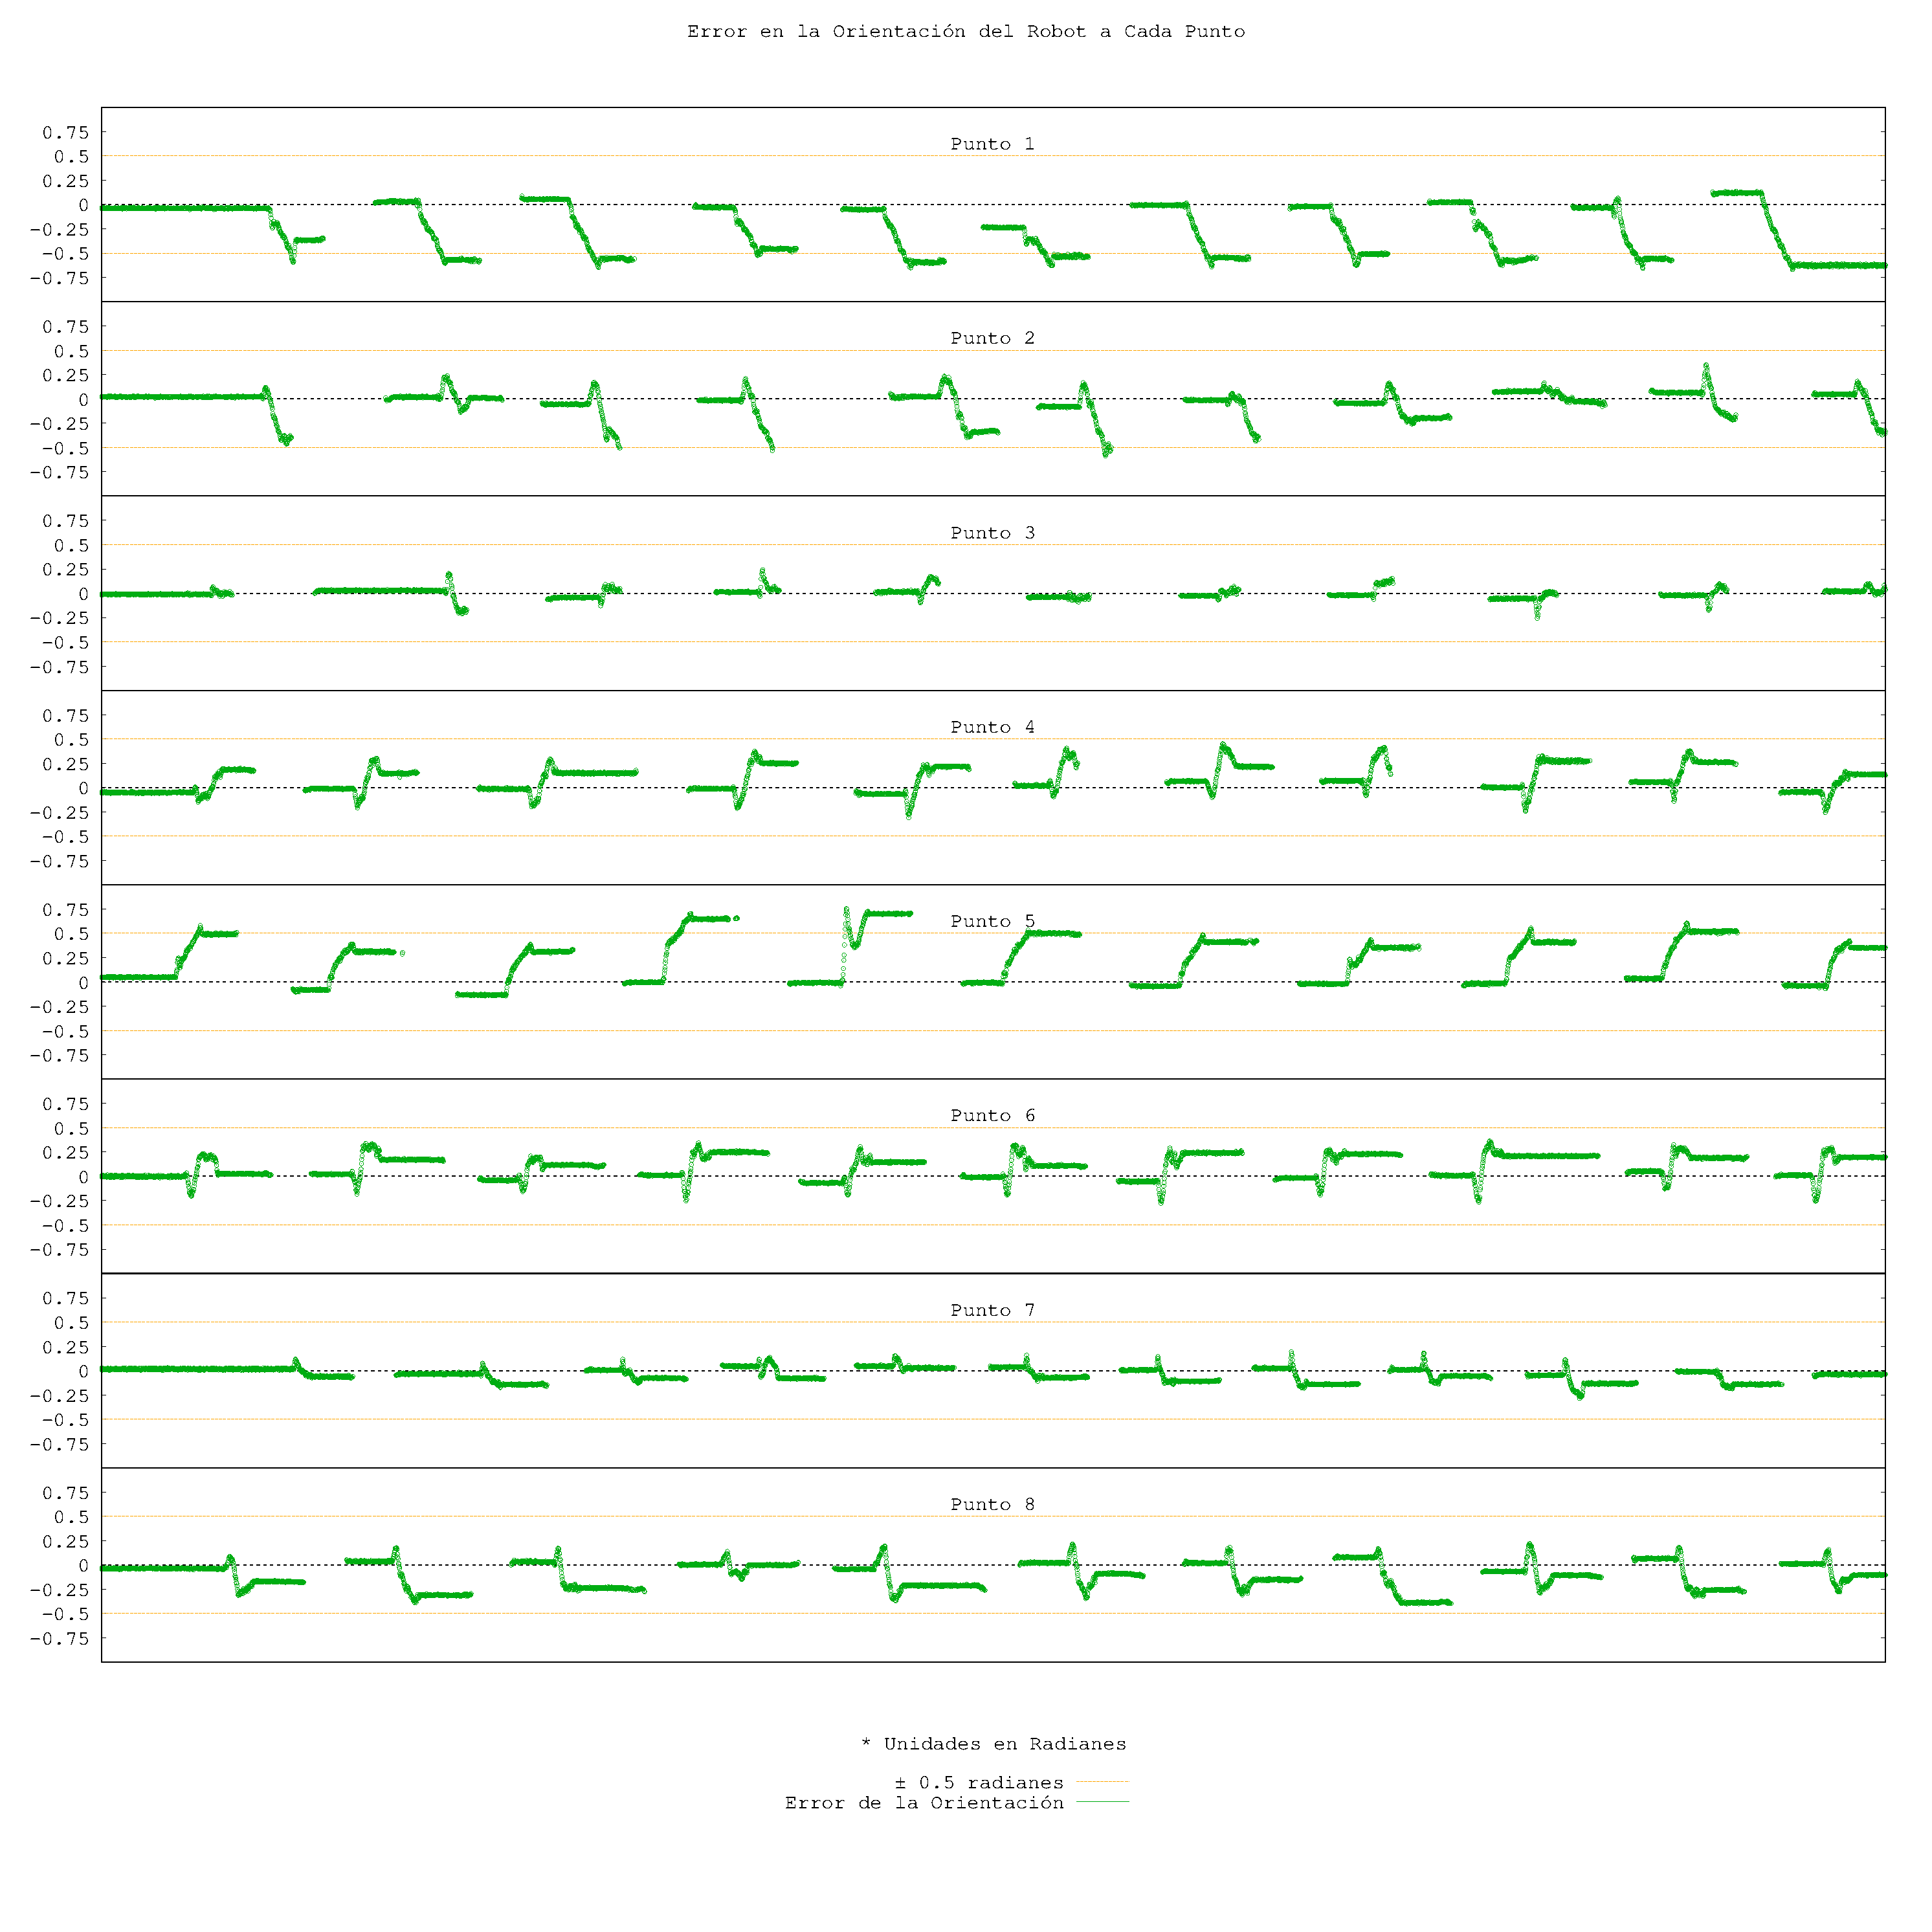
\includegraphics[height=3cm,width=8cm]{8pts260517-without_vision-multi-theta.eps}
  \caption{Error en la Orientación del Robot en las Pruebas sin Retroalimentación de Visión}
  \label{fig:orient_without_vision}
\end{figure}
%%%%%%%%%%%%%%%% end figure %%%%%%%%%%%%%%%%%%% 
%%%%%%%%%%%%%%%%%%%%%%%%%%%%%%%%%%%%%%%%%%%%%%%%%%%%%%%%%%%%%%%%%%%%%%%%%%%%%%%%%%%%%%%%
\subsection*{Pruebas con Retroalimentación de Visión y Trayectorias Dinámicas}
%%%%%%%%%%%%%%%%%%%%%%%%%%%%%%%%%%%%%%%%%%%%%%%%%%%%%%%%%%%%%%%%%%%%%%%%%%%%%%%%%%%%%%%%
El objetivo de éstas pruebas es validar el movimiento del robot ante un ambiente dinámico donde la trayectori deseada cambia rápidamente. 
\par
Para éstas pruebas se utiliza un sistema desarrollado sobre ROS con la arquitectura mostrada en la Fig. \ref{fig:ROSGral}.  El sistema de visión de SSL detecta al robot y determina su localización en el munto. A partir de ésta información, el módulo de planeación genera el siguiente punto objetivo en el mundo (para las pruebas, uno de los puntos $P_0, ..., P_8$) definidos anteriormente. La generación de rutas encuentra una ruta viable (al no existir obstáculos, la ruta siempre será una línea recta). El módulo de control genera la trayectoria para seguir la ruta generada. La trayectoria consiste en puntos intermedios entre la posición del robot y el punto objetivo. Es importante resaltar que el sistema asume que el robot no va a llegar a los puntos intermedios generados por la trayectoria ya que se actualizan antes de alcanzarlo, funcionan como \textit{puntos atractores}. El control a bajo nivel determina el vector de velocidad deseada del robot $(X, Y, \theta)$ y le envía la información al robot. La operación y algoritmos utilizados en cada módulo escapa el alcance de éste documento.
\par
El comportamiento programado para éstas pruebas consiste en que el robot (colocado inicialmente en $P_0$visite cada punto en la siguiente secuencia: $P_1, P_0, P_2, P_0, ..., P_7, P_0, P_8, P_0$. Todo de forma autónoma manteniendo la orientación del robot con dirección a $P_3$. 
\par
%%%%%%%%%%%%%%%%%%%%%%%%%%%%%%%%%%%%%%%%
\subsubsection*{Movimiento en el Plano}
%%%%%%%%%%%%%%%%%%%%%%%%%%%%%%%%%%%%%%%%
En la Fig. \ref{fig:8pts_vision_multi} se muestra la respuesta del robot en las 10 pruebas realizadas. Para cada prueba, se grafica la trayectoria deseada (generada por el módulo de control) así como la trayectoria real seguida por el robot. 
\par
Por la forma en que opera la generación de trayectorias, no se espera que todos los puntos intermedios sean alcanzados pero sí que el robot sea capaz de dirigirse a ellos creando trayectoria de forma similar a la deseada. Esto sucede en todas las pruebas realizadas, donde la trayectoria real del robot es muy similar a la deseada, alcanzando todos los puntos. En éstas pruebas se puede notar el efecto que tiene el error analizado en \ref{subsec:pruebas_sin_vision} en las trayectorias reales del robot. En los puntos en que sin visión se presenta mayor error son también a los puntos que la trayectoria se realiza con un arco más pronunciado. 
\par
%%%%%%%%%%%%%%%% begin figure %%%%%%%%%%%%%%%%%%%
\begin{figure}
  \centering
    \includegraphics[height=3cm,width=8cm]{8pts260517-with_vision-multi.eps}
  \caption{Movimiento del Robot con Retroalimentación de Visión y Trayectorias Dinámicas}
  \label{fig:8pts_vision_multi}
\end{figure}
%%%%%%%%%%%%%%%% end figure %%%%%%%%%%%%%%%%%%% 
%%%%%%%%%%%%%%%%%%%%%%%%%%%%
\subsubsection*{Orientación}
%%%%%%%%%%%%%%%%%%%%%%%%%%%%
En la Fig. \ref{fig:orient_vision_multi} se muestra el error en la orientación del robot en el tiempo para cada prueba realizada. El módulo de control considera una tolerancia para la orientación de $\pm 0.1$ radianes. El sistema no genera velocidad en $\theta$ para corregir el error si éste es menor a la tolerancia indicada. 
\par
En las 10 pruebas realizadas, el error en la orientación del robot solamente llega a 1 radian en una ocasión. En 20 ocaciones el valor absoluto del error es mayor a 0.5 radianes aunque es corregido y regresa a estar dentro del rango deseado. 
\par
%%%%%%%%%%%%%%%% begin figure %%%%%%%%%%%%%%%%%%%
\begin{figure}
  \centering
    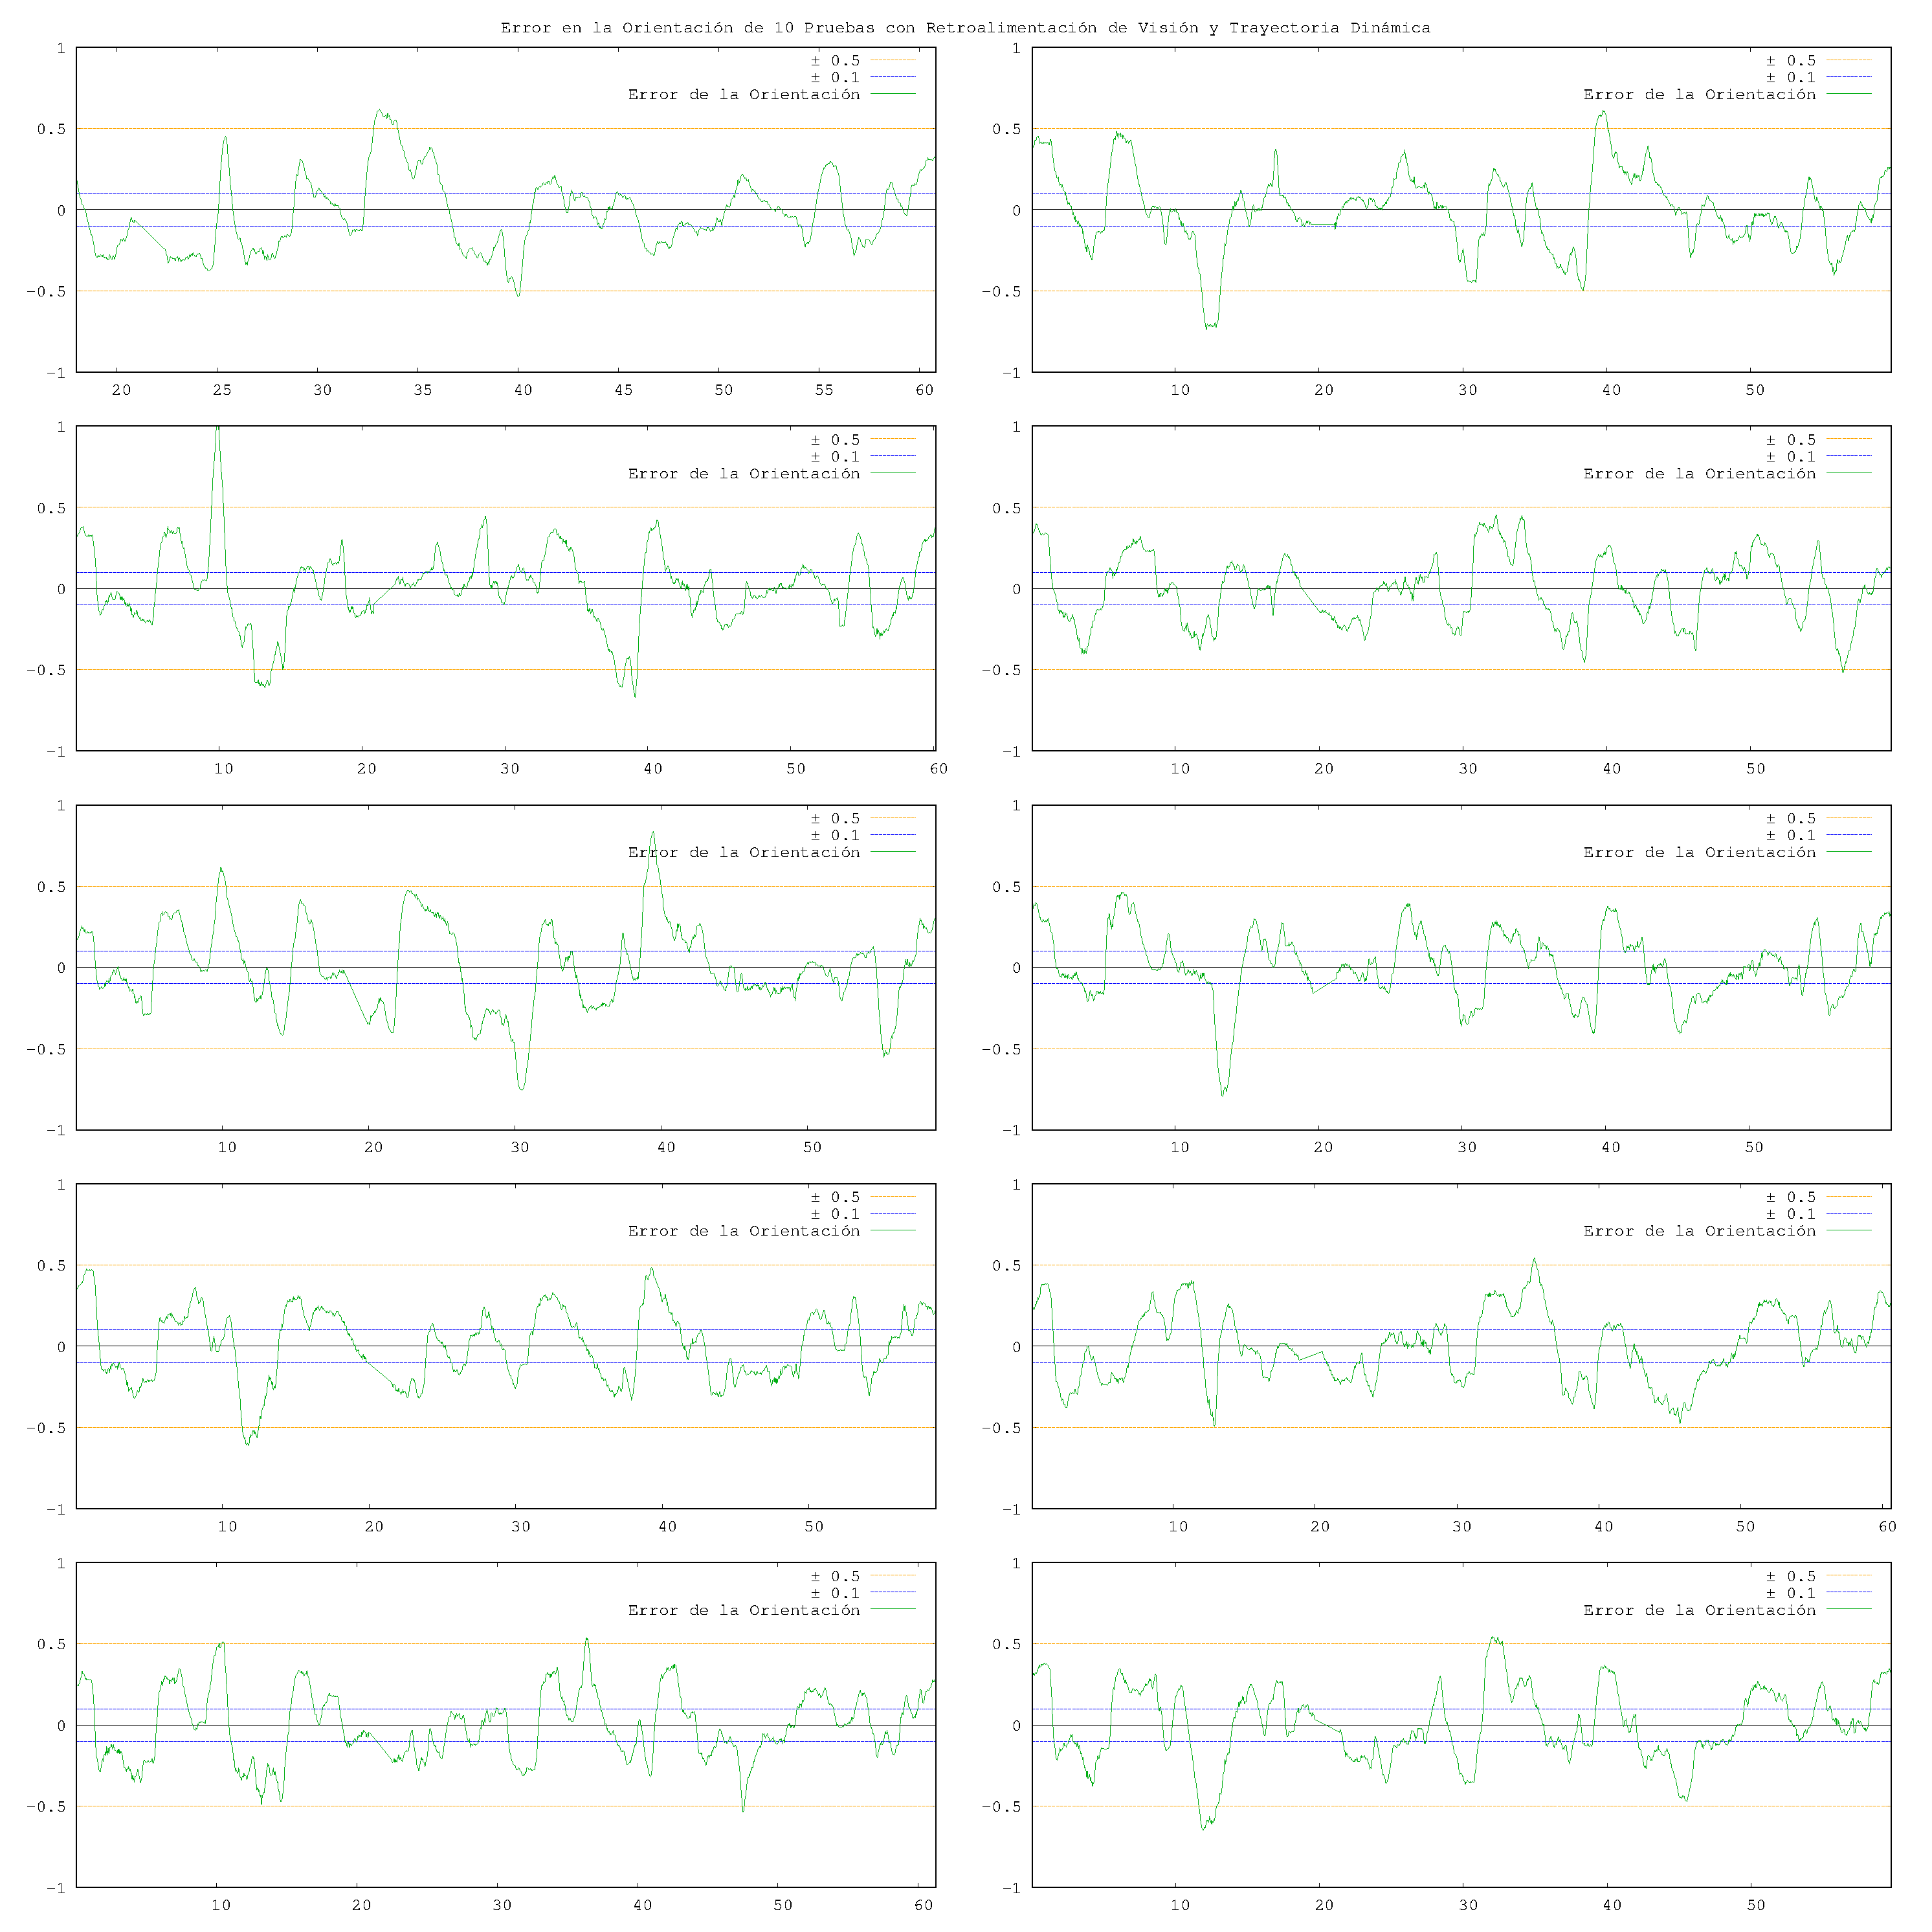
\includegraphics[height=3cm,width=8cm]{8pts260517-with_vision-multi-theta.eps}
  \caption{Velocidades Deseadas vs Velocidades Reales}
  \label{fig:orient_vision_multi}
\end{figure}
%%%%%%%%%%%%%%%% end figure %%%%%%%%%%%%%%%%%%% 
%%%%%%%%%%%%%%%%%%%%%%%%%%%%%%%%%%%%%%%%%%%%%%%%%%%%%%%%%%%%%%%%%%%%%%


%%%%%%%%%%%%%%%%%%%%%%%%%%%%%%%%%%%%%%%%%%%%%%%%%%%%%%%%%%%%%%%%%%%%%%
%%%%%%%%%%%%%%% begin table   %%%%%%%%%%%%%%%%%%%%%%%%%%
% \begin{table}[t]
% \caption{THE TABLE CAPTION USES CAPITAL LETTERS, TOO.}
% \begin{center}
% \label{table_AMRob}
% \begin{tabular}{c l l}
% & & \\ % put some space after the caption
% \hline
% Example & Time & Cost \\
% \hline
% 1 & 12.5 & \$1,000 \\
% 2 & 24 & \$2,000 \\
% \hline
% \end{tabular}
% \end{center}
% \end{table}
%%%%%%%%%%%%%%%% end table %%%%%%%%%%%%%%%%%%% 
%%%%%%%%%%%%%%%%%%%%%%%%%%%%%%%%%%%%%%%%%%%%%%%%%%%%%%%%%%%%%%%%%%%%%%

% All tables should be numbered consecutively and  captioned; the caption should use all capital letters, and centered above the table as shown in Table~\ref{table_AMRob}. The body of the table should be no smaller than 7 pt.  There should be a minimum two line spaces between tables and text.

%%%%%%%%%%%%%%%%%%%%%%%%%%%%%%%%%%%%%%%%%%%%%%%%%%%%%%%%%%%%%%%%%%%%%%
\section*{CONCLUSIONES}
Se presentó el diseño de un robot omnidireccional para su uso en aplicaciones colaborativas. La arquitectura del sistema fue probada con un robot que cumple las especificaciones de la competencia de la \emph{Small Size League} de la RoboCup, pero esta permite intercambiar componentes para otras aplicaciones gracias a su integración con el Robot Operating System.

Con el diseño propuesto se logra que el robot se mueva aproximadamente a la velocidad propuesta, manteniendo la integridad de sus componentes y con un peso menor que el contemplado inicialmente, aunque siendo capaz de cargar los 2.5 Kg propuestos. Tanto la carcasa como la base y las ruedas han sido capaces de resistir golpes entre los robots a las velocidades normales de movimiento y la visión reconoce el \textit{patrón estandar} incoporado en la carcasa. En la Fig. \ref{fig:ModRealVSdes} se muestra una comparación entre el diseño modelado en 3D y la construcción final del robot.


Como trabajo futuro se propone un método de sintonización automático para el sistema de control. Adicionalmente, es necesario expandir las capacidades del módulo de planificación para incorporar algoritmos estándar de planificación de tareas y de planificación de movimientos.


% \section*{FOOTNOTES\protect\footnotemark}
% \footnotetext{Examine the input file, asme2e.tex, to see how a footnote is given in a head.}

% Footnotes are referenced with superscript numerals and are numbered consecutively from 1 to the end of the paper\footnote{Avoid footnotes if at all possible.}. Footnotes should appear at the bottom of the column in which they are referenced.


%%%%%%%%%%%%%%%%%%%%%%%%%%%%%%%%%%%%%%%%%%%%%%%%%%%%%%%%%%%%%%%%%%%%%%
% \section*{CITING REFERENCES}

%%%%%%%%%%%%%%%%%%%%%%%%%%%%%%%%%%%%%%%%%%%%%%%%%%%%%%%%%%%%%%%%%%%%%%
% The AMRob reference format is defined in the authors kit provided by the AMRob.  The format is:

% \begin{quotation}
% {\em Text Citation}. Within the text, references should be cited in  numerical order 
% according to their order of appearance.  The numbered reference citation should be 
% enclosed in brackets.
% \end{quotation}

% The references must appear in the paper in the order that they were cited.  In addition, 
% multiple citations (3 or more in the same brackets) must appear as a `` [1-3]''.

% The bibliography style required by the AMRob is unsorted with entries appearing in the 
% order in which the citations appear. If that were the only specification, the standard 
% {\sc Bib}\TeX\ unsrt bibliography style could be used. Unfortunately, the bibliography 
% style required by the ASME has additional requirements (last name followed by first 
% name, periodical volume in boldface, periodical number inside parentheses, etc.) that 
% are not part of the unsrt style. Therefore, to get ASME bibliography formatting, you 
% must use the \verb+amrob.bst+ bibliography style file with {\sc Bib}\TeX. This file is 
% not part of the standard BibTeX distribution so you'll need to place the file someplace 
% where LaTeX can find it (one possibility is in the same location as the file being typeset).


% Here's where you specify the bibliography style file.
% The full file name for the bibliography style file 
% used for an ASME paper is asmems4.bst.
\bibliographystyle{amrob.bst}


%%%%%%%%%%%%%%%%%%%%%%%%%%%%%%%%%%%%%%%%%%%%%%%%%%%%%%%%%%%%%%%%%%%%%%

%%%%%%%%%%%%%%%%%%%%%%%%%%%%%%%%%%%%%%%%%%%%%%%%%%%%%%%%%%%%%%%%%%%%%%
% \begin{acknowledgment}
% Este trabajo fue patrocinado por la Asociación Mexicana de Cultura A.C.
% \end{acknowledgment}

%%%%%%%%%%%%%%%%%%%%%%%%%%%%%%%%%%%%%%%%%%%%%%%%%%%%%%%%%%%%%%%%%%%%%%
% The bibliography is stored in an external database file
% in the BibTeX format (file_name.bib).  The bibliography is
% created by the following command and it will appear in this
% position in the document. You may, of course, create your
% own bibliography by using thebibliography environment as in
%
% \begin{thebibliography}{12}
% % ...
% \bibitem{itemreference} D. E. Knudsen.
% {\em 1966 World Bnus Almanac.}
% {Permafrost Press, Novosibirsk.}
% % ...
% \end{thebibliography}

% Here's where you specify the bibliography database file.
% The full file name of the bibliography database for this
% article is asme2e.bib. The name for your database is up
% to you.
\bibliography{amrob.bib}

%%%%%%%%%%%%%%%%%%%%%%%%%%%%%%%%%%%%%%%%%%%%%%%%%%%%%%%%%%%%%%%%%%%%%%
\appendix       %%% starting appendix
% \section*{Appendix A: Head of First Appendix}
% Avoid Appendices if possible.

%%%%%%%%%%%%%%%%%%%%%%%%%%%%%%%%%%%%%%%%%%%%%%%%%%%%%%%%%%%%%%%%%%%%%%
% \section*{Appendix B: Head of Second Appendix}
% \subsection*{Subsection head in appendix}
% The equation counter is not reset in an appendix and the numbers will
% follow one continual sequence from the beginning of the article to the very end as shown in the following example.
% \begin{equation}
% a = b + c.
% \end{equation}

\end{document}
